\documentclass[a4paper,openany,twoside,11pt]{report}
\usepackage[utf8]{inputenc}
\usepackage[english]{babel}
\usepackage{hyperref}
\usepackage{afterpage}
\usepackage{lipsum}
\usepackage{graphicx}
\usepackage{url}
\usepackage[Algoritmo]{algorithm}
\usepackage{algorithmicx}
\usepackage{xcolor}
\usepackage{algpseudocode}
\usepackage{subcaption}
\renewcommand{\algorithmicrequire}{\textbf{Dados: }}
\renewcommand{\algorithmicensure}{\textbf{Resultado: }}
\newcommand{\blankpage}{%
    \newpage
    \null
    \thispagestyle{empty}%
    \vspace*{\fill}%
    \begin{center}%
        This page is supposed to be blank.%
    \end{center}%
    \vspace*{\fill}%
    \newpage%
}
\addto{\captionsenglish}{\renewcommand{\bibname}{References}}
\addto{\captionsenglish}{\renewcommand{\contentsname}{Table of Contents}}
\addto{\captionsenglish}{\renewcommand{\appendixname}{Appendix}}

\usepackage{xcolor}
\definecolor{codebg}{rgb}{0.95,0.95,0.97}
\definecolor{bluekeywords}{rgb}{0.00,0.25,0.65}
\definecolor{greencomments}{rgb}{0.20,0.60,0.20}
\definecolor{redstrings}{rgb}{0.75,0.00,0.15}
\definecolor{graynumbers}{rgb}{0.50,0.50,0.50}

\usepackage{listings}
\lstset{
  language=[Sharp]C,
  backgroundcolor=\color{codebg},
  basicstyle=\ttfamily\small,
  keywordstyle=\color{bluekeywords}\bfseries,
  commentstyle=\color{greencomments}\itshape,
  stringstyle=\color{redstrings},
  numberstyle=\tiny\color{graynumbers},
  numbers=left,
  numbersep=8pt,
  stepnumber=1,
  firstnumber=1,
  frame=single,
  rulecolor=\color{graynumbers},
  frameround=tttt,
  breaklines=true,
  breakatwhitespace=true,
  showstringspaces=false,
  captionpos=b,
  xleftmargin=4pt,
  xrightmargin=4pt,
  tabsize=2,
  literate={~} {$\sim$}{1}
}


\setlength{\textheight}{24.00cm}
\setlength{\textwidth}{15.50cm}
\setlength{\topmargin}{0.35cm}
\setlength{\headheight}{0cm}
\setlength{\headsep}{0cm}
\setlength{\oddsidemargin}{0.25cm}
\setlength{\evensidemargin}{0.25cm}

\title{
   \vspace{-50mm}
   \begin{minipage}[l]{\textwidth}
      \hspace{-20mm}\resizebox{75mm}{!}{\includegraphics{./img/logoISEL.png}}\\
   \end{minipage}\\[20mm]
   {\bf Hubly}
}

\author{
\begin{tabular}{ll}
             & Diogo Leitão  \\
             & Carolina Coelho \\[50mm] 
\end{tabular}}

\date{
\begin{tabular}{ll}
  {Supervisor:} & José Luís Falcão Cascalheira \\
\end{tabular}\\[10mm]
Report for the project carried out in the scope of Project and Seminar\\
Degree in Computer Science and Engineering\\[20mm]
\today}


\begin{document}
\pagenumbering{roman}
\thispagestyle{empty}
\maketitle

\baselineskip 18pt

\blankpage

\cleardoublepage
\setcounter{page}{1}
\begin{center}
\textsc{\LARGE Instituto Superior de Engenharia de Lisboa}\\[50mm]

{\large \bf  Hubly}\\[20mm]

\begin{tabular}{rl}
  51634  & Diogo Leitão\\[10mm]
           & \rule{75mm}{0.5pt}\\[5mm]
  51661  & Carolina Coelho\\[10mm]
           & \rule{75mm}{0.5pt}\\[5mm]
\end{tabular}\\[10mm]

\begin{tabular}{rl}
  Supervisor: & José Luís Falcão Cascalheira\\[10mm]
                & \rule{75mm}{0.5pt}\\[5mm]
\end{tabular}\\[10mm]

Report for the project carried out in the scope of Project and Seminar\\
Degree in Computer Science and Engineering\\[20mm]
\today\\
\end{center}

\blankpage

\chapter*{Acknowledgements}

\paragraph{}We would like to express our sincere gratitude to everyone who supported us throughout the development of this project. In particular, we are deeply grateful to our supervisor, Professor José Luís Falcão Cascalheira, for his continuous guidance, valuable feedback, and availability across the different stages of this work.

\paragraph{}We also wish to thank our teacher, Diego Gimenez Passos, for his approachability and attentiveness. His willingness to assist us, along with his insightful ideas for improvement, were instrumental to the project's progression.

\paragraph{}Furthermore, we would like to thank our families, friends, and colleagues for their unwavering support, encouragement, and understanding throughout this entire process. Their patience and motivation were essential during the most demanding periods of this endeavor.

\paragraph{}Finally, we wish to acknowledge all those who, whether directly or indirectly, contributed to the successful completion of this work.

\blankpage

\chapter*{Agradecimentos}
\paragraph{}Gostaríamos de agradecer a todos os que nos apoiaram ao longo do desenvolvimento deste projeto. Em particular, agradecemos ao nosso orientador, Professor José Luís Falcão Cascalheira, pela sua orientação, feedback e disponibilidade durante as diferentes fases do trabalho.
Gostaríamos também de agradecer às nossas famílias, amigos e colegas pelo apoio, incentivo e compreensão ao longo deste processo. A paciência e motivação foram importantes nos períodos mais exigentes do projeto.
Por fim, gostaríamos de reconhecer todos aqueles que, direta ou indiretamente, contribuíram para a conclusão deste trabalho.

\blankpage

\chapter*{Abstract}
\paragraph{}This report presents the design and implementation of Hubly, a web application developed as part of the course \textit{Project and Seminar}. The project addresses the lack of centralized information in influencer marketing workflows, where companies and digital content creators often rely on separate social networks, messaging platforms and email channels to discover contacts, negotiate collaborations and track partnership status. This fragmentation makes it difficult to compare opportunities, preserve communication context and manage multiple outreach processes in a consistent way. The proposed solution, Hubly, aims to address this limitation providing a centralized environment where users can register either as companies or as creators. Creator accounts are organized through platform-specific social profiles (for example, a YouTube or Instagram account), allowing the same creator to manage multiple profiles according to their real presence across platforms. Each social channel is represented independently, with its own audience information, content sectors and commercial conditions. Companies and creators can search for each other using criteria such as sector, platform, audience size, price range, company size and country, making the discovery process more structured and aligned with each user’s objectives. In addition, Hubly provides internal conversations associated with the relevant company or creator social profile, ensuring that communication remains linked to the context of a potential partnership. To support organizational needs, Hubly introduces collaborative team management, enabling multiple users from the same organization to manage and interact with the platform under a shared corporate account. Furthermore, to ensure transparency and system accountability, an audit logging mechanism was implemented, providing a record of critical operations performed within the application. The resulting prototype delivers a robust environment for managing company-creator interactions, reducing dependence on external channels and facilitating more organized, scalable, and transparent collaboration workflows.

\blankpage

\chapter*{Resumo}
\paragraph{}Este relatório apresenta a conceção e implementação do Hubly, uma aplicação web desenvolvida no âmbito da unidade curricular de Projeto e Seminário. O projeto aborda a falta de centralização da informação nos processos de marketing de influência, nos quais empresas e criadores de conteúdo digital recorrem frequentemente a redes sociais, plataformas de mensagens e canais de email distintos para descobrir contactos, negociar colaborações e acompanhar o estado de potenciais parcerias. Esta fragmentação dificulta a comparação de oportunidades, a preservação do contexto de comunicação e a gestão consistente de múltiplos processos de contacto.

A solução proposta, Hubly, pretende responder a esta limitação através da disponibilização de um ambiente centralizado onde os utilizadores se podem registar como empresas ou como criadores. As contas de criadores são organizadas através de perfis sociais específicos por plataforma, como, por exemplo, uma conta de YouTube ou Instagram, permitindo que o mesmo criador possa gerir vários perfis de acordo com a sua presença real nas diferentes plataformas. Cada canal social é representado de forma independente, com a sua própria informação de audiência, setores de conteúdo e condições comerciais.

Empresas e criadores podem procurar-se mutuamente utilizando critérios como setor, plataforma, dimensão da audiência, intervalo de preços, dimensão da empresa e país, tornando o processo de descoberta mais estruturado e alinhado com os objetivos de cada utilizador. Além disso, o Hubly disponibiliza conversas internas associadas à empresa ou ao perfil social do criador relevante, garantindo que a comunicação permanece ligada ao contexto de uma potencial parceria.

Para responder a necessidades organizacionais, o Hubly introduz a gestão colaborativa de equipas, permitindo que vários utilizadores da mesma organização possam gerir e interagir com a plataforma através de uma conta corporativa partilhada. Adicionalmente, para assegurar transparência e responsabilidade no sistema, foi implementado um mecanismo de registo de auditoria, que permite manter um histórico de operações críticas realizadas na aplicação.

O protótipo resultante disponibiliza um ambiente estruturado para a gestão de interações entre empresas e criadores, reduzindo a dependência de canais externos e facilitando processos de colaboração mais organizados, escaláveis e transparentes.

\tableofcontents
\listoffigures
\lstlistoflistings

%\listoftables


\setcounter{page}{1}
\pagenumbering{arabic}

\chapter{Introduction}

\paragraph{}Due to the extreme growth of social networks and the necessity for businesses to maintain a strong digital presence, combined with the importance for influencers and content creators to effectively monetize their audience through multiple platforms, managing partnerships has become highly complex. Currently, most of these collaborations involve a high fragmentation of communication channels, scattering interactions across \textit{Instagram DMs}, \textit{WhatsApp}, \textit{Google Forms}, \textit{Gmail}, and \textit{Telegram}\dots Reaching out to content creators has consequently become a chaotic process, making it incredibly difficult for startups and brands to track and organize marketing partnerships. This difficulty in finding direct contact methods and maintaining control over negotiation statuses was the primary motivation behind the development of the Hubly project.

The Hubly project aims to develop an easy-to-use and intuitive marketplace application that allows users to maintain full control over their influencer marketing campaigns, promoting structured business workflows and improving partnership organization, while simultaneously helping them find the best match to work with. In the context of this application, a creator is not treated as a single entity, instead, the platform operates through social profiles, which act as granular extensions where the user can manage campaigns based on specific metrics like follower counts, custom sectors, and pricing. Multiple users, such as distinct brands or individual creators, can discover each other and establish direct communication channels within a dedicated, professional networking environment.

\section{Functional Requirements}
\paragraph{}This section outlines the core functional requirements of the application, which focuses on connection, discovery, and communication management between companies and digital creators. The following entities define the system's core functionality:

\begin{itemize}
    \item \textbf{User Registration:} Users must complete a comprehensive registration process that includes providing accurate personal information.
    \begin{itemize}   
        \item \textbf{User:} An individual who accesses and uses the platform. Users can register, log in, and manage their authentication credentials. Since this application is private and secure, access is strictly restricted to authenticated users with a verified email address. After the initial registration, a user must establish their identity as either a \emph{Creator} or a \emph{Company}.    
        
        \item \textbf{Creator:} A user type representing content creators or influencers. A creator profile includes an artistic name, verification status, availability status, algorithmic global rating based on reviews, statistics about chats, and historical response metrics. Each creator can register and manage multiple individual \emph{Social Profiles} across different platforms.
        
        \begin{itemize}
        
            \item \textbf{Social Profile:} A granular, platform-specific representation of a creator's presence (e.g., YouTube, Instagram, TikTok). Each profile is linked to a specific platform, public username, direct link, and target audience metrics (such as follower count). It also defines customized commercial constraints, including minimum and maximum pricing tiers, and is classified under specific content sectors.
        
        \end{itemize}
        
        \item \textbf{Company:} A user type representing brands, agencies, or startups looking for marketing partnerships. A company profile contains the legal or commercial name, description, corporate size, website link, and country of headquarters. Like creators, companies map their operations to specific industry sectors. By operating as a company, users gain the advantage of having their history tracked and processed to customize the application experience through tailored ecosystem recommendations.
    
    \end{itemize}

    \item \textbf{Email Confirmation:} Users must confirm their email address during the registration process to ensure the validity of their contact information.

    \item \textbf{Sector:} A classification system used to group both company operations and creator social profiles into specific market niches (e.g., Finance, Tech, Fashion, Gaming). This shared taxonomy enables accurate, cross-referenced discovery and high-compatibility matches during searches.
    
    \item \textbf{Rating System:} A feedback mechanism that allows companies and creators to rate digital creators based on previous interactions or partnership experiences. These ratings provide insights into a creator's reliability, professionalism, communication quality, and overall performance. This system contributes to the platform's transparency and helps users make informed decisions when selecting creators for future collaborations.
    
    \item \textbf{Verification System:} A process that allows users to verify their identity and authenticity on the platform. This system enhances trust and credibility by confirming that users are who they claim to be, which is particularly important for creators seeking partnerships with companies. Verified users may receive a special badge or status on their profiles, signaling their legitimacy to potential partners.

    \item \textbf{Search Engine:} An advanced, multi-criteria discovery mechanism allowing targeted, paginated queries. The engine processes inputs distinctly based on the target entity data models:
    \begin{itemize}
        \item \textbf{Creator Search:} Utilizes a paginated model (\emph{CreatorSearchInputModel}) to filter profiles by platform identification (\texttt{PlatformId}), username keywords (\texttt{PlatformUserName}), specific follower brackets (\texttt{FollowersCountMin} and \texttt{FollowersCountMax}), pricing budget constraints (\texttt{PriceMin} and \texttt{PriceMax}), matching sector tags (\texttt{Sectors}), and dynamic page size control (\texttt{Page} and \texttt{PageSize}).
        \item \textbf{Company Search:} Utilizes a paginated model (\emph{CompanySearchInputModel}) to filter corporate entities by corporate name keywords (\texttt{Name}), a list of associated business sectors (\texttt{Sectors}), workforce size categories (\texttt{CompanySize}), countries of headquarters (\texttt{Countries}), and dynamic page size control (\texttt{Page} and \texttt{PageSize}).
    \end{itemize}
    
    \item \textbf{Conversation \& Messaging:} A secure internal chat architecture initiated directly between a company and a creator's specific \emph{Social Profile} rather than a generic user account. This structure ensures context-specific negotiations. The chat system logs real-time messages, tracks message read status metrics per participant, and supports message editing and deletion.
    
    \item \textbf{Private Tag System:} A productivity management tool that allows users to independently organize their active conversations. Users can create custom workflow tags with designated names and hexadecimal colors. These tags can be secretly assigned to conversations to track private negotiation statuses (e.g., \emph{Contacted}, \emph{Negotiation}, \emph{Accepted}, \emph{Rejected}) without the counterparty's knowledge, directly mitigating outreach confusion.
    
    \item \textbf{Profile Views History:} An analytical tracking mechanism that logs whenever an authenticated user views a company profile or a creator's specific social profile, providing critical transparency metrics regarding platform exposure and interest trends.

    \item \textbf{Recommendation Engine:} An intelligent system that analyzes user behavior, preferences, and interactions to provide personalized suggestions for companies and creators, enhancing the overall user experience and facilitating more effective partnerships.

\end{itemize}
 

\section{Report Structure}

\paragraph{}This report is organized into the following chapters:

Chapter \textbf{\ref{ch:similar_systems}} explores the strengths and shortcomings of similar systems and influencer marketplaces currently available on the market.

Chapter \textbf{\ref{ch:architecture}} presents the overall design and structure of the Hubly project, describing its main components, the interaction between different layers, and how the web interfaces connect with the backend API and the central entities of companies and creators. Here we also talk about the technologies used and the reasons for their choice.

Chapter \textbf{\ref{ch:backend}} focuses on the backend component of the project, explaining its architecture, routing mechanisms, and the implementation details of key functionalities such as messaging pipelines and DTO processing.

Chapter \textbf{\ref{ch:database}} focuses on the database component of the project, explaining its relational schema definitions, constraints, and the implementation details of data persistence.

Chapter \textbf{\ref{ch:frontend_web}} presents the web interface of the application, explaining the implementation of important features.

Chapter \textbf{\ref{ch:tests}} focuses on the tests we performed on the project to ensure the correctness, reliability, and security of the application.

Finally, Chapter \textbf{\ref{ch:conclusion}} summarizes the final thoughts on the work done along with the future work that could be implemented to further expand the Hubly ecosystem for the startup market.
\chapter{System requirements}\label{ch:system_requirements}

\section{Functional Requirements}
\paragraph{}This section outlines the core functional requirements of the application, which focuses on connection, discovery, and communication management between companies and digital creators. The following entities define the system's core functionality:

\begin{itemize}
    \item \textbf{User Registration:} Users must complete a comprehensive registration process that includes providing accurate personal information.
    \begin{itemize}   
        \item \textbf{User:} An individual who accesses and uses the platform. Users can register, log in, and manage their authentication credentials. Since this application is private and secure, access is strictly restricted to authenticated users with a verified email address. After the initial registration, a user must establish their identity as either a \emph{Creator} or a \emph{Company}.    
        
        \item \textbf{Creator:} A user type representing content creators or influencers. A creator profile includes an artistic name, verification status, availability status, algorithmic global rating based on reviews, statistics about chats, and historical response metrics. Each creator can register and manage multiple individual \emph{Social Profiles} across different platforms.
        
        \begin{itemize}
        
            \item \textbf{Social Profile:} A granular, platform-specific representation of a creator's presence (e.g., YouTube, Instagram, TikTok). Each profile is linked to a specific platform, public username, direct link, and target audience metrics (such as follower count). It also defines customized commercial constraints, including minimum and maximum pricing tiers, and is classified under specific content sectors.
        
        \end{itemize}
        
        \item \textbf{Company:} A user type representing brands, agencies, or startups looking for marketing partnerships. A company profile contains the legal or commercial name, description, corporate size, website link, and country of headquarters. Like creators, companies map their operations to specific industry sectors.
    
    \end{itemize}

    \item \textbf{Email Confirmation:} Users must confirm their email address during the registration process to ensure the validity of their contact information.

    \item \textbf{Sector:} A classification system used to group both company operations and creator social profiles into specific market niches (e.g., Finance, Tech, Fashion, Gaming). This shared taxonomy enables accurate, cross-referenced discovery and high-compatibility matches during searches.
    
    \item \textbf{Rating System:} A feedback mechanism that allows companies and creators to rate digital creators based on previous interactions or partnership experiences. These ratings provide insights into a creator's reliability, professionalism, communication quality, and overall performance. This system contributes to the platform's transparency and helps users make informed decisions when selecting creators for future collaborations.
    
    \item \textbf{Verification System:} A process that allows users to verify their identity and authenticity on the platform. This system enhances trust and credibility by confirming that users are who they claim to be, which is particularly important for creators seeking partnerships with companies. Verified users may receive a special badge or status on their profiles, signaling their legitimacy to potential partners.

    \item \textbf{Search Engine:} An advanced, multi-criteria discovery mechanism allowing targeted, paginated queries. The engine processes inputs distinctly based on the target entity data models:
    \begin{itemize}
        \item \textbf{Creator Search:} Utilizes a paginated model (\emph{CreatorSearchInputModel}) to filter profiles by platform identification (\texttt{PlatformId}), username keywords (\texttt{PlatformUserName}), specific follower brackets (\texttt{FollowersCountMin} and \texttt{FollowersCountMax}), pricing budget constraints (\texttt{PriceMin} and \texttt{PriceMax}), matching sector tags (\texttt{Sectors}), and dynamic page size control (\texttt{Page} and \texttt{PageSize}).
        \item \textbf{Company Search:} Utilizes a paginated model (\emph{CompanySearchInputModel}) to filter corporate entities by corporate name keywords (\texttt{Name}), a list of associated business sectors (\texttt{Sectors}), workforce size categories (\texttt{CompanySize}), countries of headquarters (\texttt{Countries}), and dynamic page size control (\texttt{Page} and \texttt{PageSize}).
    \end{itemize}
    
    \item \textbf{Conversation \& Messaging:} A secure internal chat architecture initiated directly by a company or a creator's specific \emph{Social Profile} rather than a generic user account. This structure ensures context-specific negotiations. The chat system logs real-time messages, tracks message read status metrics per participant, and supports message editing and deletion.
    
    \item \textbf{Private Tag System:} A productivity management tool that allows users to independently organize their active conversations. Users can create custom workflow tags with designated names and hexadecimal colors. These tags can be secretly assigned to conversations to track private negotiation statuses (e.g., \emph{Contacted}, \emph{Negotiation}, \emph{Accepted}, \emph{Rejected}) without the counterparty's knowledge, directly mitigating outreach confusion.
    
    \item \textbf{Profile Views History:} An analytical tracking mechanism that logs whenever an authenticated user views a company profile or a creator's specific social profile, providing critical transparency metrics regarding platform exposure and interest trends.

    \item \textbf{Recommendation Engine:} An intelligent system that analyzes user behavior, preferences, and interactions to provide personalized suggestions for companies and creators, enhancing the overall user experience and facilitating more effective partnerships.

\end{itemize}

\chapter{Similar Systems} \label{ch:similar_systems}

Influencer marketing management is a rapidly evolving area in the software industry, with several platforms available on the market offering tools to help brands discover creators, track campaign metrics, and establish professional partnerships. This chapter presents a brief comparative analysis of two notable applications in this sector — Collab Only and Influencity — highlighting their strengths, technical inspirations, and architectural limitations in relation to Hubly.

The goal of this comparison is to understand how these existing solutions address common influencer management needs and to identify critical gaps that Hubly aims to fill, particularly in terms of platform flexibility, advanced search capabilities, active user intent, granular multi-profile organization, and dedicated internal communication frameworks.

\section{Collab Only}
Collab Only is a niche marketplace application in the influencer marketing sector designed to connect brands and creators through a mutual interest matching model. Operating with a mobile-first approach, it utilizes an interface heavily inspired by matchmaking applications (such as Tinder), where a potential connection is established only after both a company and a creator swipe positively on each other's profiles based on initial registration data.

From a functional standpoint, Collab Only introduces a highly valuable business concept regarding partnership classification. It allows users to specify the explicit nature of the collaboration they are seeking, categorizing them into distinct operational models:
\begin{itemize}
    \item \textbf{Affiliate Marketing:} Performance-based partnerships where creators earn commissions on sales.
    \item \textbf{One-time Ad:} Short-term sponsorships or dedicated single posts for immediate campaign reach.
    \item \textbf{Strategic Partner:} Long-term brand ambassadorships and ongoing marketing relationships.
    \item \textbf{And More...}

\end{itemize}
This precise classification of partnership models represents an excellent business data structure that Hubly recognizes as a high-value asset to be integrated and refined within its own business model.

However, a deep technical and operational analysis of Collab Only reveals major structural limitations that hinder its adoption in real-world startup workflows:
\begin{itemize}
    \item \textbf{Absence of an Active Search Engine:} The application completely lacks a manual search or filtering mechanism. Connections rely entirely on an automated, static recommendation feed generated upon account creation. This design wrongly assumes that companies and creators have static requirements, completely blocking users from dynamically altering their search intents or running target-specific market queries.
    \item \textbf{Lack of Native Chat Infrastructure:} Despite forcing a matching mechanism, the platform fails to provide a robust internal chat engine tailored for contract negotiations between companies and influencers, forcing users to migrate their communications off-platform immediately after a match occurs.
    \item \textbf{Monolithic Account Constraints:} The platform does not allow a creator to register and manage multiple standalone sub-profiles for each of their social channels (e.g., separating YouTube metrics from Instagram metrics). This lack of granular database architecture leads to a complete disorganization of data, making it impossible to manage platform-specific pricing or audience scales independently.
\end{itemize}

In summary, while Collab Only introduces an innovative approach by defining distinct partnership types, its overall execution remains unpractical for professional use due to low market adoption, the rigid absence of a multi-criteria search engine, and a lack of data organization for multi-channel creators. 

\section{Influencity}
Influencity is widely considered an industry-leading platform in the influencer marketing ecosystem, boasting an established market presence with millions of indexed profiles. It serves as an enterprise-grade software-as-a-service (SaaS) designed to provide companies with robust data-driven metrics. 

From a technical and architectural standpoint, Influencity serves as an excellent reference and inspiration for the future scaling of Hubly. Its infrastructure relies heavily on the integration of native social media Graph APIs (such as Meta Graph API and YouTube Data API). Through these programmatic connections, the platform automatically retrieves, synchronizes, and audits real-time metrics. Furthermore, by requesting administrative access tokens from consenting users, it unlocks deep analytical insights regarding target audiences. This allows companies to evaluate high-value demographic data, including:
\begin{itemize}
    \item average audience age brackets and distribution tiers,
    \item geographic distribution and top countries of origin,
    \item gender audience ratios and engagement authenticity metrics.
\end{itemize}
This layer of deep audience intelligence represents an invaluable technological asset that demonstrates how API-driven data processing can maximize the value proposition of a marketing application.

However, a critical evaluation of Influencity’s operational mechanics reveals significant structural vulnerabilities and architectural limitations:
\begin{itemize}
    \item \textbf{Data-Mining vs. Active Marketplace Intent:} A common misconception is that the millions of creators searchable on Influencity are active users looking for deals. In reality, the platform operates as an automated indexing tool (similar to an advanced corporate database or automated spreadsheet) that lists creators regardless of their actual intent to collaborate. The platform lacks a bilateral intent structure, meaning companies often waste resources reaching out to creators who are inactive or closed to brand deals.
    \item \textbf{High Financial and Complexity Barriers:} The platform is exclusively focused on enterprise-level budgets, completely alienating early-stage startups and small businesses due to prohibitive pricing models.
    \item \textbf{Communication Isolation and Platform Fragmentation:} Influencity focuses entirely on the discovery and analytical vetting phases. It does not centralize communication flows, missing a robust, profile-anchored internal chat infrastructure or a private negotiation CRM pipeline. Just like using traditional outreach, brands must extract the scraped contact data and revert to fragmented external channels (such as individual corporate emails or direct messaging apps) to execute negotiations.
    \item \textbf{Rigid Social Ecosystem Constraints:} The platform is structurally restricted to a limited selection of legacy social networks (Instagram, YouTube, and TikTok). It lacks the modular flexibility to integrate emerging or alternative content channels, limiting its long-term adaptability.
\end{itemize}

In summary, while Influencity represents a peak technical standard for audience data analysis via native APIs, its lack of user intent centralization and failure to mitigate communication fragmentation leaves a massive opening in the mid-market. 

\section{Chapter Synthesis}
By analyzing both systems, a clear market polarization becomes evident. On one hand, Collab Only attempts to build a bilateral marketplace but fails due to its oversimplified, rigid matchmaking mechanics and lack of essential technical features like search engines and proper data structures. On the other hand, Influencity provides an incredibly powerful, API-driven analytical engine, but operates purely as a cold, enterprise-grade data-mining spreadsheet, completely ignoring communication management and user collaboration intent. 

Hubly capitalizes on these exact market failures. By combining the high-intent, dual-sided community model of a marketplace with the professional rigor of a paginated, multi-criteria search engine, profile-specific chat systems, and a private negotiation CRM pipeline, Hubly bridges the gap between raw data analysis and structured workflow management, creating a practical and accessible alternative for the modern startup ecosystem.

\chapter{Architecture}\label{ch:architecture}
\paragraph{}This chapter presents the architecture of Hubly, describing the main components of the system and the way they interact. The system is organized as a web application composed of a browser-based frontend, a backend API, a relational database and a reverse proxy responsible for routing incoming requests. The implementation details of the backend, database model and frontend are described in the chapters \ref{ch:backend}, \ref{ch:database} and \ref{ch:frontend_web} respectively.
Figure \ref{fig:architecture} illustrates the main architectural components of Hubly and their communication paths.

\begin{figure}[H]
    \centering
    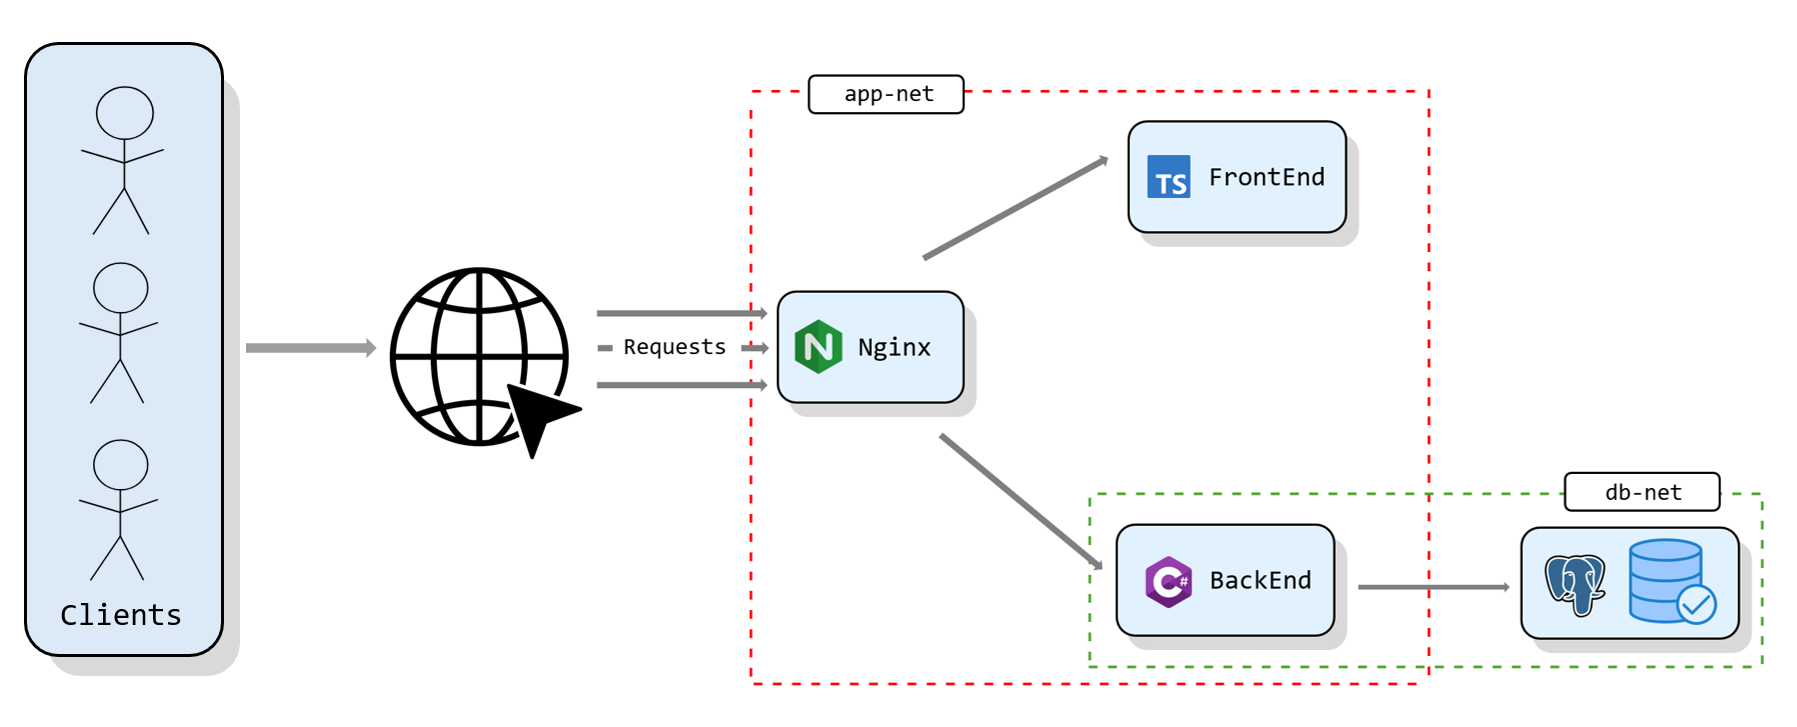
\includegraphics[width=0.85\textwidth]{img/general_structure.png}
    \caption{Hubly system Architecture}
    \label{fig:architecture}
\end{figure}

\section{Architecture Overview}

\paragraph{}Hubly follows a client-server architecture. Users interact with the system through a web browser, which loads the frontend application and sends requests to the backend API. The backend is responsible for processing application operations, enforcing business rules and accessing persistent data stored in the relational database.

A reverse proxy is placed between the browser and the internal application services. Its role is to receive incoming HTTP requests and route them to the appropriate component. Requests related to the web interface are forwarded to the frontend application, while API requests are forwarded to the backend service. The backend is the only component that communicates directly with the database.

This organization separates the user interface, application logic and data persistence concerns. It also allows each component to be developed, deployed and maintained independently, while keeping the communication between components explicit and controlled.


\section{System Components}

\paragraph{}This section describes the main components of Hubly and their role in the overall architecture.

\subsection{Reverse Proxy}
\paragraph{}The reverse proxy is implemented using Nginx~\cite{nginx} and acts as the entry point for incoming requests. Its purpose is to route requests to the appropriate internal service according to the requested path.

Requests associated with the web interface are forwarded to the frontend application. Requests targeting the API, such as those using the /api path, are forwarded to the backend service. This component allows the frontend and backend services to remain internal to the application environment while exposing a single access point to the browser.

\subsection{Frontend}
\paragraph{}The frontend application is the user-facing component of Hubly. It is executed through the user’s web browser and provides the interface used to access the main application workflows, such as registration, profile management, search and messaging.

The frontend was developed using React~\cite{react} and Next.js~\cite{nextjs}. Its main responsibility is to render the user interface, collect user input and send HTTP requests to the backend API when application data is required or modified. The frontend does not access the database directly. All data operations are performed through the backend service.

In the containerized environment, the frontend runs in the hubly-web container and communicates with the reverse proxy through the app-net network.

\subsubsection{Technologies used in Frontend}
\paragraph{}Table~\ref{tab} summarizes the main technologies and libraries used in the frontend component of Hubly. These technologies support the implementation of the web interface, component structure, styling, state management, API communication.

\begin{table}[H]
\centering
\small
\begin{tabular}{|p{0.22\textwidth}|p{0.32\textwidth}|p{0.36\textwidth}|}
\hline
\textbf{Technology} & \textbf{Purpose} & \textbf{Use in Hubly} \\ \hline
React~\cite{react} & JavaScript library for building user interfaces based on reusable components. & Used to implement the frontend pages, interface components and client-side interaction logic. \\ \hline
Next.js~\cite{nextjs} & React framework that provides routing and support for server-side rendering and application structure. & Used to organize the web application routes, layouts and page structure. \\ \hline
TypeScript~\cite{typescript} & Statically typed superset of JavaScript. & Used to define typed data structures, component properties and service interfaces, reducing type-related errors during development. \\ \hline
Shadcn/UI & Component collection built on top of Radix UI and Tailwind CSS. & Used as the basis for several interface components, providing a consistent structure for forms, dialogs, buttons and other UI elements. \\ \hline
Radix UI~\cite{radixui} & Library of accessible, unstyled UI primitives. & Used to support interactive components such as dialogs, dropdowns and tabs. \\ \hline
Tailwind CSS~\cite{tailwindcss} & Utility-first CSS framework for styling web interfaces. & Used to define the visual layout and styling of the frontend components. \\ \hline
Lucide React~\cite{lucidereact} & Icon library for React applications. & Used to include SVG icons in the user interface. \\ \hline
TanStack React Query~\cite{reactquery} & Library for fetching, caching and synchronizing server state. & Used to manage data obtained from the backend API, reducing repeated requests and simplifying loading and error states. \\ \hline
SignalR~\cite{signalr} & Library for real-time communication between client and server. & Used in the messaging component to receive updates related to conversations and messages. \\ \hline
js-cookie~\cite{jscookie} & JavaScript library for handling browser cookies. & Used to support client-side access to cookie-related information required by the frontend flow. \\ \hline
\end{tabular}
\caption{Frontend technologies used in Hubly}
\label{tab}
\end{table}

\subsection{Backend}
\paragraph{}The backend API is responsible for processing the operations requested by the frontend. It implements the application logic related to users, companies, creators, social profiles, search, conversations, tags, ratings and recommendations.

The backend was developed using ASP.NET Core~\cite{aspnetcore} and exposes a REST API consumed by the frontend application. It also performs authentication and authorization checks, validates business rules and coordinates access to persistent data. Database operations are abstracted through Entity Framework Core, preventing the frontend from interacting directly with the database.

In the containerized environment, the backend runs in the hubly-api container. It belongs to both app-net and db-net, allowing it to receive requests from the reverse proxy and communicate with the database service.

\subsubsection{Technologies used in Backend}
\paragraph{}Table~\ref{tab:backend_technologies} summarizes the main technologies and libraries used in the backend component of Hubly. These technologies support the implementation of the REST API, data access, authentication, content validation, email confirmation, object mapping and backend testing.

\begin{table}[H]
\centering
\small
\begin{tabular}{|p{0.24\textwidth}|p{0.31\textwidth}|p{0.35\textwidth}|}
\hline
\textbf{Technology} & \textbf{Purpose} & \textbf{Use in Hubly} \\ \hline
ASP.NET Core~\cite{aspnetcore} & Framework for developing web APIs in the .NET ecosystem. & Used to implement the backend API, define HTTP endpoints and process requests from the frontend application. \\ \hline
Entity Framework Core~\cite{entityframeworkcore} & Object-relational mapper for .NET applications. & Used to access the PostgreSQL database through C\# domain entities and repository operations. \\ \hline
PostgreSQL~\cite{postgreSql} & Relational database management system. & Used to persist the main data of the system, including users, companies, creators, social profiles, conversations, messages, tags and ratings. \\ \hline
BCrypt.Net-Next~\cite{bcrypt} & Library for password hashing. & Used to store password validation information without persisting plain-text passwords. \\ \hline
Profanity Detector~\cite{profanitydetector} & Library for detecting inappropriate terms in text. & Used to validate user-generated textual content before it is stored. \\ \hline
Mapster~\cite{mapster} & Object mapping library for .NET. & Used to transform domain entities into response models exposed by the API. Listing~\ref{lst:mapster-controller} shows an example of this transformation. \\ \hline
MailKit~\cite{mailkit} & .NET library for sending and receiving emails through standard mail protocols. & Used to send email confirmation codes during the registration process. \\ \hline
SignalR~\cite{signalr} & Library for real-time communication between server and clients. & Used by the backend to support real-time updates in the messaging component. \\ \hline
xUnit~\cite{xunit} & Testing framework for .NET applications. & Used to implement backend unit and integration tests. \\ \hline
Testcontainers~\cite{testcontainers} & Library for creating temporary Docker containers during tests. & Used to run integration tests with an isolated PostgreSQL database environment. \\ \hline
\end{tabular}
\caption{Backend technologies used in Hubly}
\label{tab:backend_technologies}
\end{table}

\begin{lstlisting}[caption={Concise domain-to-DTO transformation}, label={lst:mapster-controller}]
// Mapping a single entity to a response model
return res.Match(
success => Ok(success.Adapt(<CompanyOutputModel>)),
error => error switch { /* ... */ }
);

// Mapping a collection of items during search
Items = success.Items.Adapt<List>(),
\end{lstlisting}

\subsection{Database}

\paragraph{}The database component is responsible for storing the persistent data used by the system. Hubly uses a PostgreSQL~\cite{postgreSql} relational database to store information about users, companies, creators, social profiles, sectors, conversations, messages, tags, ratings, authentication data and profile-view history.

The database is not directly accessible from the frontend or from the browser. All interactions with the database are performed by the backend API. In the containerized environment, the database runs in the hubly-db container and is connected only to the db-net network.

This separation limits direct access to the database service and keeps data management concentrated in the backend layer.

\section{Deployment and Network Organization}

\paragraph{}The system is executed in a containerized environment, where each main component runs in a separate container. This organization separates the frontend application, backend API, reverse proxy and database into independent services.

Nginx acts as the entry point for incoming HTTP requests. Requests related to the web interface are forwarded to the frontend application, while requests targeting the API, such as those using the \texttt{/api} path, are forwarded to the backend service.

The containerized environment uses two Docker networks:

\begin{enumerate}
\item \textbf{\texttt{app-net}:} This network connects the reverse proxy, frontend and backend services. It is used for routing requests between the browser-facing entry point and the internal application services.

\item \textbf{\texttt{db-net}:} This network connects the backend service to the PostgreSQL database. The database is not directly accessed by the frontend or by the browser; all database operations are performed through the backend API.

\end{enumerate}

This separation makes the communication paths between components explicit and limits direct access to the database service. It also allows the application services to be configured and executed independently during development and deployment.



\chapter{Backend}\label{ch:backend}
\paragraph{}This chapter presents the backend components of the project, focusing on the structural organization of the API and the implementation of its main functionalities.

\section{Backend Architecture}

\begin{figure}[H]
\centering
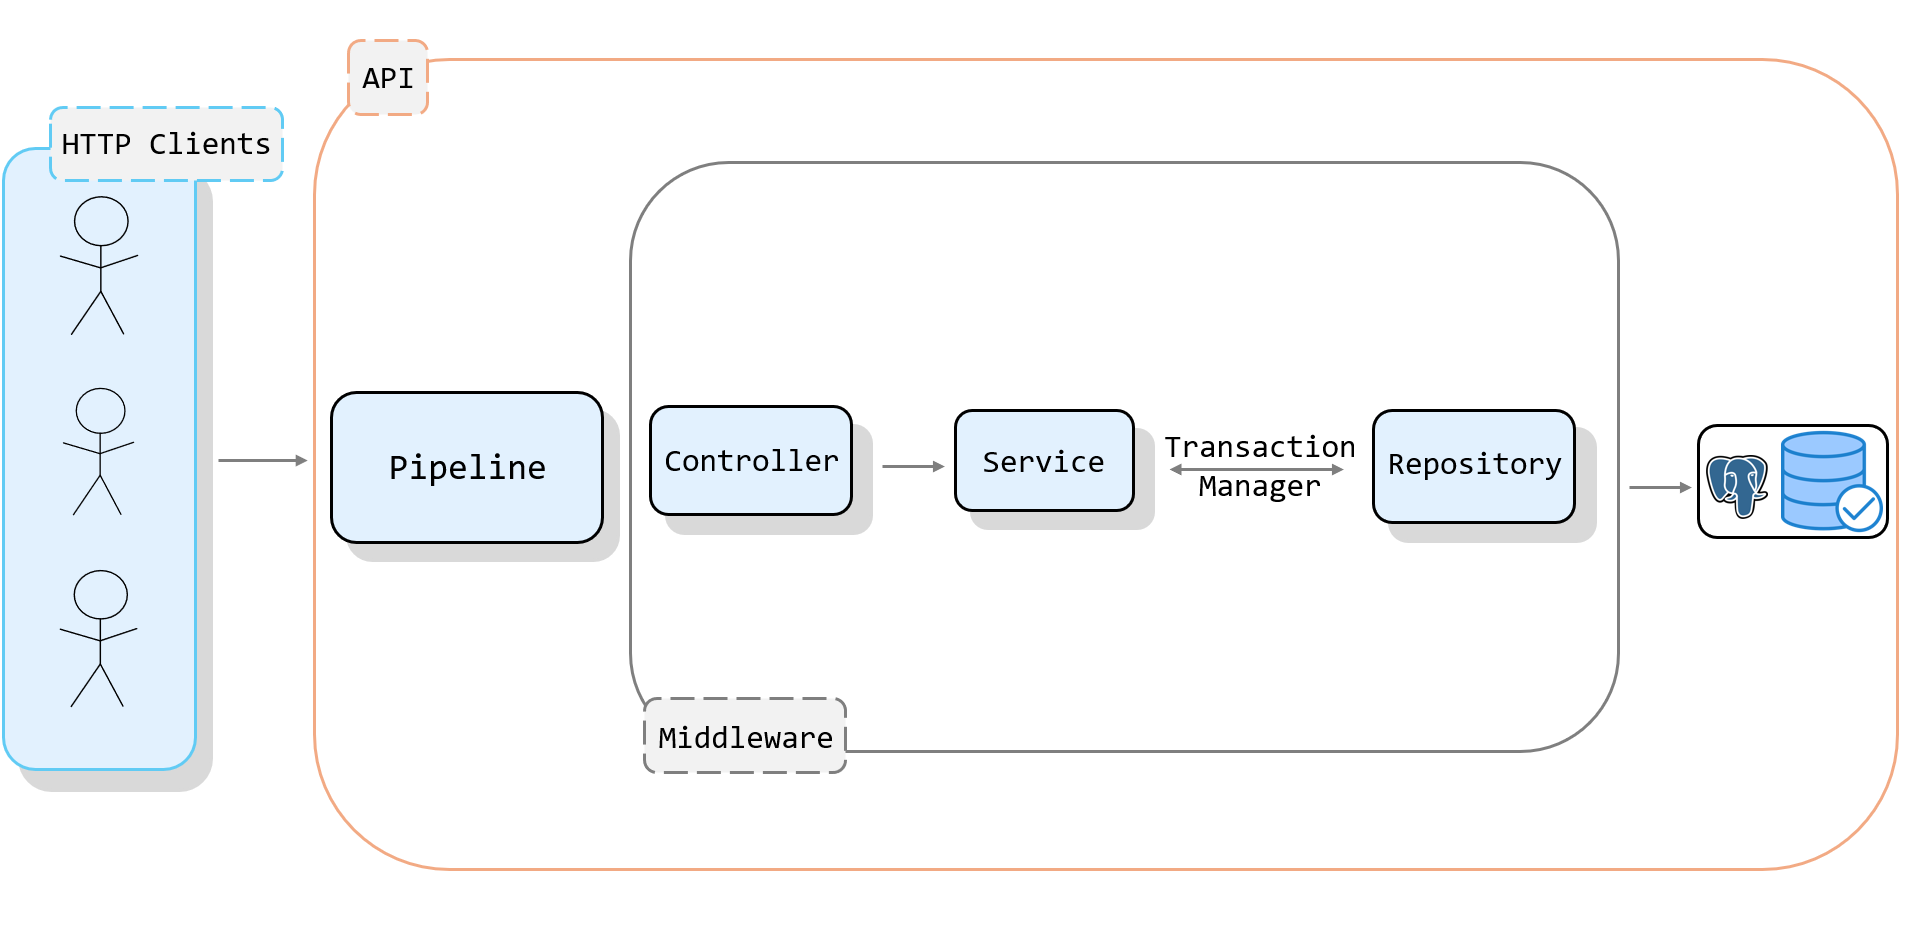
\includegraphics[width=1.05\textwidth]{img/API_structure.png}
\caption{API Architecture Overview}
\label{fig:api-structure}
\end{figure}

\subsection{Design Principles and Patterns}

To ensure robustness in error management, our API adopts the Problem Details for HTTP APIs standard (RFC 9457) \cite{rfc9457}. This specification allows the backend to communicate errors through structured, consistent responses, replacing ambiguous exceptions with clear, machine-readable diagnostic information.

The backend is organized into distinct layers to promote maintainability, scalability, and a strict separation of concerns. This modular approach allows for the isolated development and evolution of different system components:

\begin{itemize}
\item \textbf{Controllers}: Act as the entry point, managing incoming HTTP requests and orchestrating the appropriate responses.
\item \textbf{Services}: Encapsulate the core business logic, ensuring that domain rules are applied independently of the presentation layer.
\item \textbf{Repositories}: Define the data access layer, abstracting database interactions and shielding the business logic from persistence-specific details.
\end{itemize}

Furthermore, to uphold data consistency and integrity across complex operations, we implemented a \textbf{Transaction Manager}. This component ensures the atomicity of database interactions by grouping multiple operations into a single logical unit. Consequently, all operations within a transaction are committed only if entirely successful; otherwise, the system triggers a rollback, effectively preventing the database from entering an inconsistent state.

\subsection{Authentication and Authorization Interceptors}

To enforce security across our API, most endpoints are protected by an interception mechanism that validates not only user authentication but also the status of their account. Specifically, our system requires that every request originates from an authenticated user who has successfully verified their email address.

To streamline this, we implemented an \texttt{AuthenticatedUser} class that serves as a specialized parameter in controller actions. When a method signature includes this parameter, our interceptor system automatically triggers, performing a two-fold validation:
\begin{enumerate}
\item It verifies the integrity and validity of the authentication token or cookie provided in the request.
\item It confirms the user’s account status, ensuring that their email address has been verified.
\end{enumerate}

If either validation fails—whether the credentials are invalid or the email remains unconfirmed—the interceptor intercepts the execution flow and returns an appropriate error response following the Problem Details format, preventing the controller logic from ever being reached.

This design offers several architectural advantages:
\begin{itemize}
\item \textbf{Centralized Logic}: Authentication and authorization rules are consolidated within a single component, eliminating code duplication across controllers.
\item \textbf{Separation of Concerns}: Controller actions remain strictly focused on business logic, decoupled from security or identity verification.
\item \textbf{Declarative Security}: Security requirements are explicitly declared through method signatures, making the codebase easier to audit.
\item \textbf{Unified Mechanism}: The same interception pipeline transparently supports both token-based (mobile) and cookie-based (web) authentication.
\end{itemize}

Figure~\ref{fig:interceptor-functioning} illustrates the operational flow of this mechanism. When credentials are valid and the user is verified, the \texttt{AuthenticatedUser} object is populated with the user’s identity, allowing the request to proceed. Otherwise, the request is rejected with a descriptive error response, ensuring the system remains protected.

\begin{figure}[H]
\centering
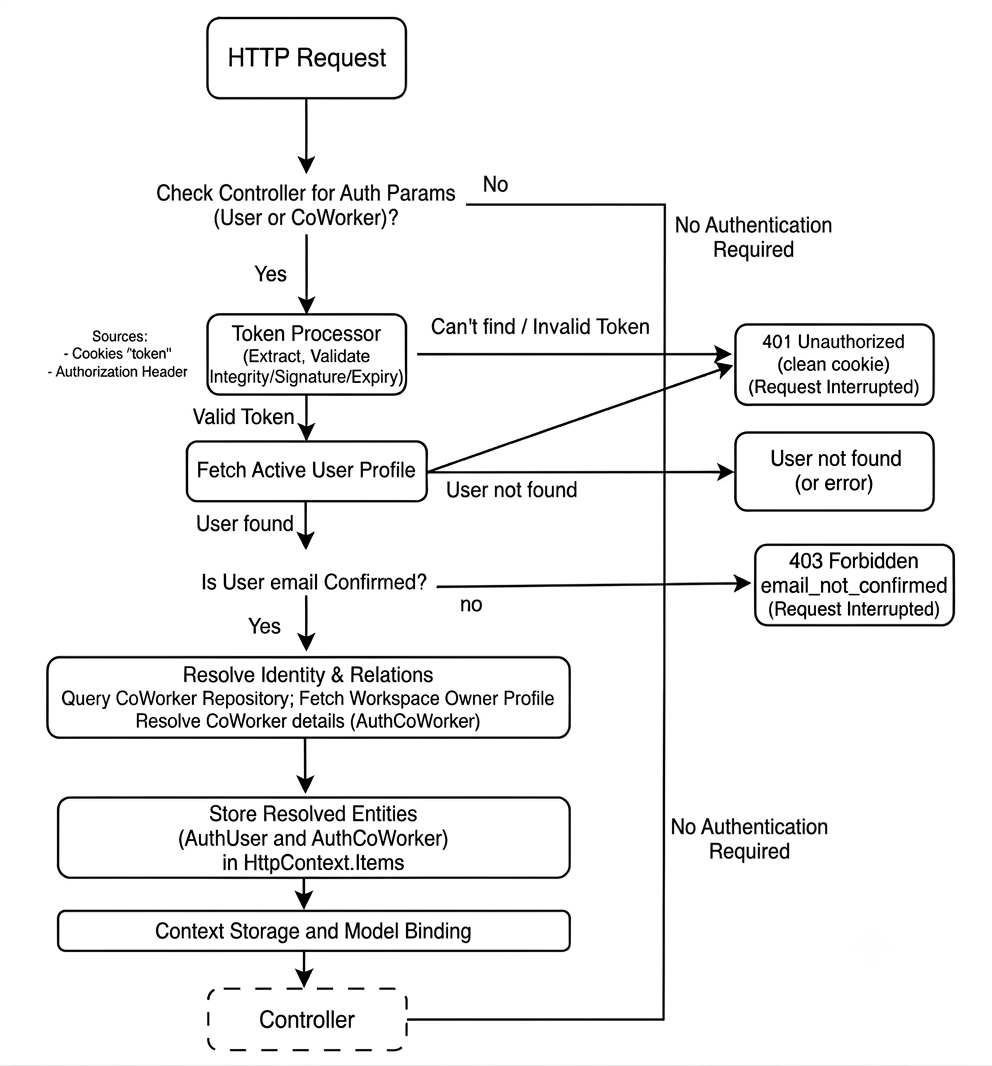
\includegraphics[width=10cm]{img/interceptor_functioning.png}
\caption{Authentication Interceptor Workflow}
\label{fig:interceptor-functioning}
\end{figure}

This pattern ensures a clean, maintainable, and highly secure boundary between security enforcement and business operations.

\subsection{Error Handling Middleware}

A cornerstone of our error management strategy is the global error-handling middleware, which serves as a protective layer between the core application logic and the client-side response. This component is designed to ensure that unexpected faults are captured and communicated in a standardized, predictable manner.

\begin{lstlisting}[caption={Error Handling Middleware Implementation}, label={lst:error-handling-middleware}]
private static async Task HandleExceptionAsync(HttpContext context, Exception exception)
{
var statusCode = (int)HttpStatusCode.InternalServerError;
context.Response.ContentType = "application/problem+json";
context.Response.StatusCode = statusCode;

    var problem = ProblemResponse.InternalServerError;

    var json = JsonSerializer.Serialize(problem);
    await context.Response.WriteAsync(json);
}
\end{lstlisting}

As illustrated in Listing~\ref{lst:error-handling-middleware}, this middleware fulfills two primary architectural roles:

\begin{itemize}
\item \textbf{Global Exception Interception}: It acts as a safety net, capturing any unhandled exceptions during request execution—such as database connectivity issues or unforeseen system failures. By intercepting these faults, the middleware prevents raw or sensitive stack trace information from propagating to the client, which significantly hardens the API against information disclosure.

\item \textbf{Standardized Response Mapping}: The middleware transforms intercepted exceptions into well-defined responses conforming to the \texttt{application/problem+json} format (RFC 9457). This ensures that error reporting remains consistent across the entire system, providing clients with a reliable and easily consumable interface for handling failures.
\end{itemize}

Technically, the implementation enforces a 500 Internal Server Error status code by default for unhandled faults. It then serializes a predefined ProblemResponse object into JSON, ensuring the output adheres strictly to our established API error contract, thereby maintaining seamless communication with the frontend.


\subsection{Email Service}

The system incorporates a dedicated email service primarily to orchestrate user identity verification. By requiring users to validate their registration via a unique verification code, we significantly enhance platform security and ensure that all accounts are linked to accessible, legitimate email addresses.

The verification workflow operates as follows:
\begin{itemize}
\item \textbf{Token Generation}: Upon registration, the system automatically generates a unique, time-sensitive verification code.
\item \textbf{Secure Dispatch}: The email service transmits this code to the user's provided email address.
\item \textbf{Identity Confirmation}: The user is required to input the received code within the application to finalize the account activation process.
\end{itemize}

Figure~\ref{fig:email-service-structure} illustrates the internal architecture of the email service and its integration with the core system components.

\begin{figure}[H]
\centering
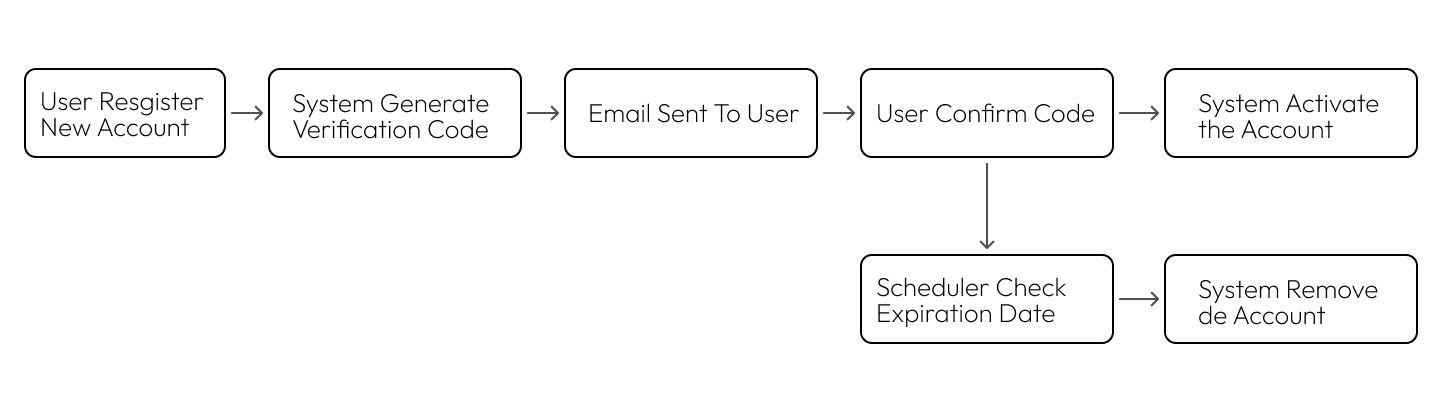
\includegraphics[width=1.05\textwidth]{img/email_service_structure.png}
\caption{Email Service Architectural Overview}
\label{fig:email-service-structure}
\end{figure}

By maintaining this structured approach to identity verification, the email service serves as a cornerstone for maintaining a clean and trustworthy user base within the application ecosystem.

\subsection{Authentication Pipeline}

To ensure that only authorized users can access protected resources, we implemented a robust authentication pipeline. This mechanism is responsible for validating user credentials and account status before any business logic is executed within the controller actions.

Architecture of the Authentication Pipeline
The authentication process is enforced through a custom filter, RequireAuthenticationAttribute, which integrates into the ASP.NET Core request lifecycle. This attribute works in conjunction with a TokenProcessor service, forming a centralized validation pipeline:

\begin{enumerate}
\item \textbf{Identity Resolution}: The pipeline retrieves the authentication token either from the request headers or the application cookies.
\item \textbf{Token Validation and Identity Mapping}: The TokenProcessor validates the token and resolves the user's identity, ensuring that the session is active and legitimate.
\item \textbf{Authorization and Account Status Check}: Beyond verifying the token, the pipeline explicitly checks the \texttt{IsEmailConfirmed} flag. If the account is not verified, the system terminates the request and returns a \texttt{403 Forbidden} status, mandating email confirmation to proceed.
\item \textbf{Dependency Injection}: Once the user is authenticated and verified, the pipeline populates the \texttt{HttpContext.Items} with an \texttt{AuthenticatedUser} object. This object is then automatically injected into controller actions via a custom AuthenticatedUserModelBinder, allowing for clean and declarative parameter access.
\end{enumerate}

Cookie Configuration and Security
For web-based interactions, the application utilizes secure cookie-based session management. Listing~\ref{lst:login-response} illustrates the configuration used to persist the authentication session:

\begin{lstlisting}[caption={Authentication Cookie Configuration}, label={lst:login-response}]
var cookieOptions = new CookieOptions
{
HttpOnly = true,
Secure = false, // Must be true in production
SameSite = SameSiteMode.Strict,
Expires = DateTime.Now.AddDays(7)
};
Response.Cookies.Append("token", tokenValue, cookieOptions);
\end{lstlisting}

This configuration adheres to security best practices:
\begin{itemize}
\item \textbf{HttpOnly}: Renders the cookie inaccessible to client-side scripts, effectively preventing Cross-Site Scripting (XSS) attacks.
\item \textbf{SameSite (Strict)}: Instructs the browser to only send the cookie with requests originating from our domain, providing a robust defense against Cross-Site Request Forgery (CSRF).
\item \textbf{Expiration Policy}: Sets a persistent 7-day session, which is dynamically maintained and refreshed upon valid user interaction.
\end{itemize}

By decoupling security validation from business logic through this custom pipeline, we ensure that authentication requirements are explicitly declared via method signatures, resulting in a cleaner, more secure, and highly maintainable codebase.
\section{Backend Key Functionalities}

\subsection{User Management and Authentication}
\paragraph{}The user management module is responsible for account-related operations, including user registration, authentication, email confirmation and profile-related interactions. In addition to basic operations (CRUD) over user data, this module includes mechanisms for password handling, session management and email verification.

\subsubsection{Identity and Authentication}
\paragraph{}Authentication is handled through a token-based mechanism. The system includes the following mechanisms:
\begin{itemize}
    \item \textbf{Secure Password Handling}: Passwords are not stored in plain text. A dedicated \texttt{IPasswordEncoder} is used to generate password validation information based on hashing and salt.
    \begin{itemize}
        \item \textbf{Why Hashing and Salt?}: When a user registers or authenticates, a cryptographic hashing function transforms the plaintext password into a unique, fixed-length, and irreversible string, making it mathematically unfeasible to reconstruct the original password if the data is intercepted. To elevate this security standard, a dynamic \textit{salt}, a unique, random string is appended to each password prior to the hashing process. This ensures that even if multiple users choose the exact same password, their final stored hashes will be completely distinct from one another, effectively neutralizing dictionary attacks and pre-computed rainbow table compromises.
    \end{itemize}
    \item \textbf{Token Management}: The system manages user sessions by limiting the number of active tokens per user. When the limit is reached, the system automatically invalidates the oldest session, maintaining a balanced token lifecycle.
    \item \textbf{Email Verification}: To ensure user authenticity, the registration process triggers an asynchronous email confirmation flow. This uses a numeric code generator with a strictly defined expiration policy, enforced by the persistence layer.
\end{itemize}

\subsection{Transactional Integrity}
\paragraph{}A defining characteristic of our backend is the use of an \textbf{Atomic Transaction Manager}. Operations such as registration, password changes and email verification are executed within transactional contexts when they require multiple database changes. 
This ensures that actions such as creating a user record, generating an initial confirmation code, and updating security metadata are executed as a single unit of work. If one of the operations fails, the transaction is rolled back, avoiding partial updates. This approach is further reinforced by the \textit{OneOf} functional pattern, which forces explicit error handling for every business rule violation (e.g., duplicate emails, invalid credentials), providing predictable API responses.

\subsection{Multi-Criteria Search}
\paragraph{}The backend implements search mechanisms that allow users to query companies and creator social profiles using multiple criteria. The search logic is separated into two input models, one for creator social profiles and one for companies. Both models support pagination and filters adapted to the corresponding entity.
\begin{itemize}
    \item \textbf{Creator social profile search (\texttt{CreatorSearchInputModel}):} This model filters creator social profiles according to information associated with each specific platform profile. It processes inputs such as platform identification (\texttt{PlatformId}), username keywords (\texttt{PlatformUserName}), granular audience sizing (\texttt{FollowersCountMin} and \texttt{FollowersCountMax}), commercial budget constraints (\texttt{PriceMin} and \texttt{PriceMax}), and specific market niches (\texttt{Sectors}), all encapsulated within an optimized pagination controller (\texttt{Page} and \texttt{PageSize}). To safeguard platform reputation, this discovery layer incorporates a peer-reviewed rating system with built-in mathematical validation to strictly prevent self-rating bias.
    \item \textbf{Company search (\texttt{CompanySearchInputModel}):} Designed for creators seeking brand partnerships, this filters organizations by corporate name keywords (\texttt{Name}), active industrial or business sectors (\texttt{Sectors}), workforce scaling categories (\texttt{CompanySize}), and geographic parameters (\texttt{Countries}), utilizing matching pagination rules.
\end{itemize}

\subsection{Messaging and Conversation Architecture}
\paragraph{}The conversation module supports communication between users within the system.
\begin{itemize}
    \item \textbf{Participant Model}: Conversations support different participant types (Company vs. Creator Social Profile, Creator Social Profile vs. Creator Social Profile, Company vs. Company) through a flexible participant model, ensuring the conversation context is correctly mapped to the entity performing the action.
    \item \textbf{Conversation Management:} The system stores message state information and supports synchronization between participants.
        \begin{itemize}
            \item \textit{Message Lifecycle States:} When a participant edits a message, the system updates an \texttt{is\_edited} boolean flag to true, signaling the frontend to display an "edited" badge to both users, maintaining transparency. Similarly, message deletion utilizes a soft-delete pattern, turning the \texttt{is\_deleted} flag to true instructs the frontend to stop rendering the message content, ensuring privacy while maintaining database auditability.
            \item \textit{Unread Message Counting:} The system computes unread message counts per participant, allowing the frontend to display this information in the user interface.
            \item \textit{Background Read Synchronization:} Before a user even fully enters a conversation view, the architecture pre-evaluates and synchronizes the session state in the background against the ID of the last sent or received message. This information allows the system to determine which messages have already been read.
            \item \textit{Real-Time State Tracking:} Leveraged via native SignalR client integrations, the platform enables bidirectional web socket functionality. This updates the chat layout instantly with message states, edits, or incoming deliveries in real-time as other participants interact, completely eliminating the need for manual browser refreshes.
        \end{itemize}
    \item \textbf{Organization through Tagging}: The system allows users to create and assign private tags to conversations.Tags can be used by each user to organize conversations according to their own workflow.
    \begin{itemize}
    \item \textit{Default tags:} Out of the box, the database seeds a set of standard, industry-specific operational tags designed to map traditional partnership pipelines. These include:
    \begin{itemize}
        \item \texttt{Contacted} (Hex: \texttt{\#3498db}) — Signifies initial outreach.
        \item \texttt{Negotiating} (Hex: \texttt{\#f1c40f}) — Indicates active discussion.
        \item \texttt{Accepted} (Hex: \texttt{\#2ecc71}) — Marks a successful match and partnership agreement.
        \item \texttt{Rejected} (Hex: \texttt{\#e74c3c}) — Partnership rejection.
    \end{itemize}
    \item \textit{Custom tags:} If the default tags do not fit a user's workflow, the system allows the user to create additional tags by defining a name and a hexadecimal color code.
    \item \textit{Private visibility:} Tag assignments are private to the user who creates or assigns them. For example, when a user marks a conversation as \texttt{Negotiating} or \texttt{Rejected}, that classification is only visible to that user. The other participant does not have access to these private tags.
\end{itemize}
\end{itemize}

\subsection{History Tracking and Recommendations}
\paragraph{}The backend stores profile-view history and uses this information, together with previous search parameters, to support recommendation features. This feature allows the system to generate dashboard recommendations using information from previous profile views and search parameters, helping users discover companies or creator social profiles related to their past interactions.
\subsubsection{Recommendation Workflow}

\paragraph{}The system records profile-view events whenever a user opens a company profile or a creator social profile. This information, together with previous search parameters, is used as input for the recommendation process. The recommendation behavior differs depending on the type of entity being recommended. Figure~\ref{fig:recommendation-system} illustrates the logic behind this process.

\begin{itemize}
\item \textbf{Company recommendations:} When a user searches for companies, the search parameters can be stored and later used to recommend company profiles with similar characteristics. These characteristics may include sectors, headquarters country and company size.
\item \textbf{Creator social profile recommendations:} When a user searches for creator social profiles, the search criteria can also be stored for later use. The recommendation function can use criteria such as platform, sectors, audience size and price range to return creator social profiles related to previous searches.
\end{itemize}

\begin{figure}[H]
    \centering
    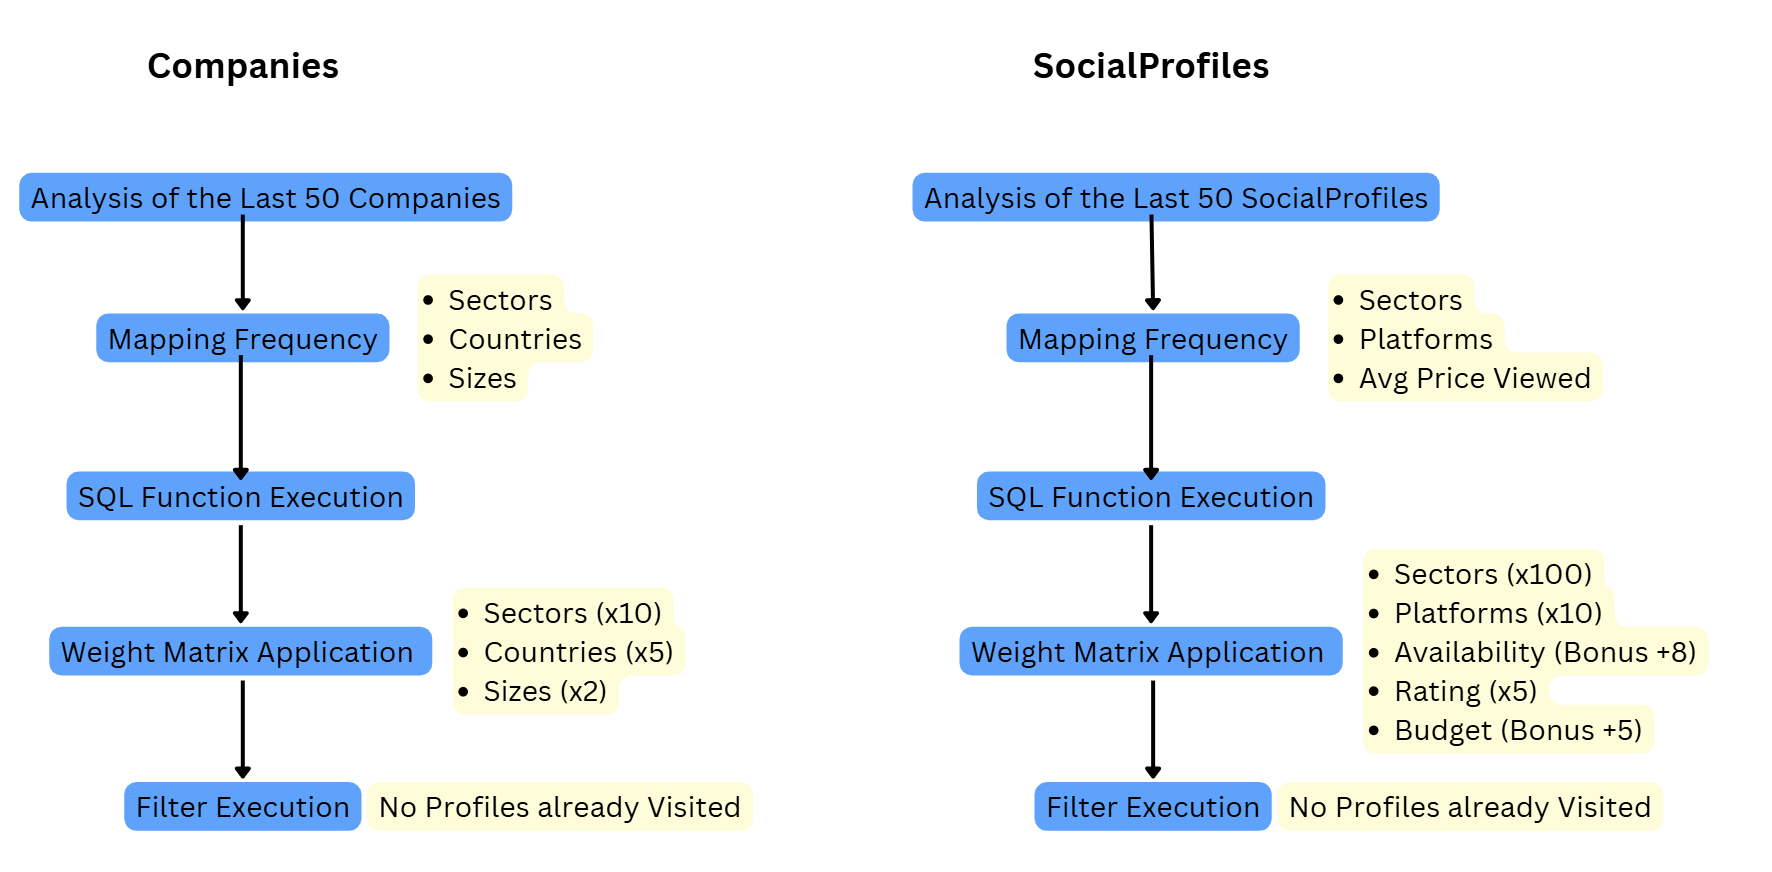
\includegraphics[width=0.95\textwidth]{./img/Recomendation_System.png}
    \caption{Recommendation System Architecture}
    \label{fig:recommendation-system}
\end{figure}


\subsection{Collaborative Coworking Framework}
\paragraph{}The Collaborative Coworking Framework enables multi-user access to a shared workspace without requiring the sharing of credentials. This mechanism establishes an operational hierarchy separating the workspace owner (administrator) from invited operators.

\subsubsection{Pipeline Integration and Context Resolution}
\paragraph{}As outlined in the request pipeline analysis, the coworker state is evaluated before the request reaches the application logic. The \texttt{RequireAuthenticationAttribute} filter and the \texttt{TokenProcessor} resolve the execution context by extracting the operator details into an \texttt{AuthenticatedCoWorker} instance, while simultaneously identifying the workspace owner as an \texttt{AuthenticatedUser}. Both objects are stored within the \texttt{HttpContext.Items} dictionary and mapped via custom model binding to be available at the controller level.

\subsubsection{Service Layer Abstraction and Audit Logging}
\paragraph{}Past the API controller layer, the underlying business services and the persistence layer operate independently of the specific identity that initiated the request. Data mutations, campaign configurations, and state updates are processed within the scope of the primary administrator's workspace identity.

\paragraph{}This design isolates core domain logic from identity validation rules, allowing the coworker to execute updates on behalf of the administrator. Because the service layer processes these changes within the context of the workspace owner, tracking individual actions within a shared workspace requires a decoupled tracking mechanism. To ensure accountability and record which physical identity performed each state modification, the architecture incorporates a dedicated Audit Logging system, as detailed in the following section.


\begin{figure}[ht]
    \centering
    \makebox[\textwidth][c]{
        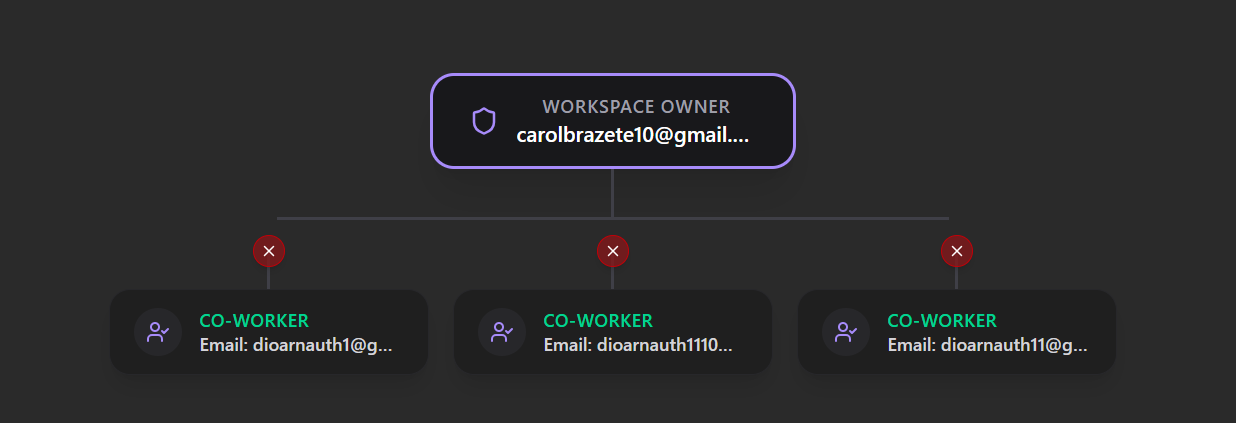
\includegraphics[width=0.95\textwidth]{./img/Team_Hierarchy_Admin.png}
    }
    \caption{Team Hierarchy - Admin Vision}
    \label{fig:team-hierarchy}
\end{figure}

\begin{figure}[ht]
    \centering
    \makebox[\textwidth][c]{
        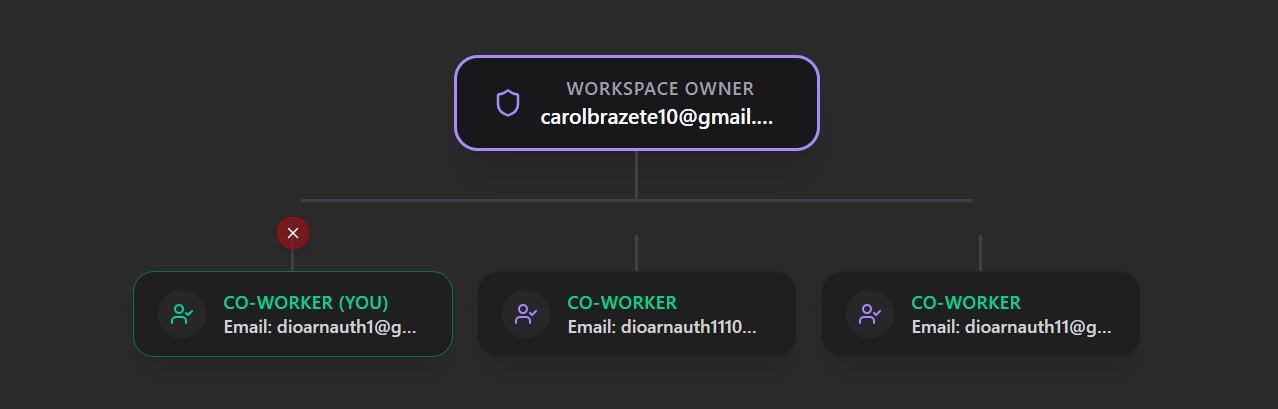
\includegraphics[width=0.95\textwidth]{./img/Team_Hierarchy_CoWorker.png}
    }
    \caption{Team Hierarchy - CoWorker Vision}
    \label{fig:team-hierarchy}
\end{figure}

\subsection{Asynchronous Audit Logging Architecture}
\paragraph{}To ensure operational accountability within shared multi-user workspaces, the platform incorporates a generalized, decoupled audit logging architecture. This framework isolates the responsibility of tracking system state changes from the primary request-execution threads, preventing administrative monitoring from introducing performance overhead or blocking user interactions.

\subsubsection{Execution Lifecycle and Queue Ingestion}
\paragraph{}The logging framework is integrated directly within the core business service layer, executing alongside the application's domain logic. When a service processes a state-changing operation, it aggregates the relevant execution metadata—such as identifiers for both the workspace owner (\texttt{UserId}) and the active operator (\texttt{CoWorkerId})—into an \texttt{AuditEntry} structure.

\paragraph{}This entry encapsulates the specific action name along with a contextual data payload resolved during the execution workflow. Once constructed, the \texttt{AuditEntry} is dispatched directly to an in-memory storage component managed by the \texttt{AuditQueue} class. This dispatch marks the transition of the audit record from the synchronous application workflow into an isolated, asynchronous processing pipeline.

\subsubsection{Asynchronous Processing and Deferred Persistence}
\paragraph{}Once an item is successfully queued, its subsequent formatting and physical database persistence are handled independently by a background infrastructure layer. The \texttt{AuditBackgroundProcessor} class operates as a long-running hosted service by extending the framework's native \texttt{BackgroundService}, continuously monitoring the queue via non-blocking asynchronous operations.

\paragraph{}Upon retrieving an entry from the queue, the processor establishes a transient dependency injection scope (\texttt{IServiceProvider.CreateScope}) to isolate the operation from any active HTTP context lifecycle. The background processing then executes the following phases:
\begin{itemize}
    \item \textbf{Reflection-Based Interpolation:} The metadata is routed through the \texttt{IAuditService} to the \texttt{AuditFormatter} utility, which uses reflection mechanisms to dynamically inspect the properties of the generic payload object.
    \item \textbf{Template Resolution:} The extracted parameters are mapped onto a static dictionary of predefined text templates, substituting structural placeholders with the actual runtime values of the operation to construct a human-readable description.
\end{itemize}
\paragraph{}Following this interpolation phase, the service instantiates the final \texttt{AuditLog} domain entity, appends a coordinated universal timestamp (\texttt{DateTime.UtcNow}), and performs a database write operation through the \texttt{IAuditRepository} to persist the historical record.
\chapter{Database Model}\label{ch:database}

This chapter details the database model designed for the collaborative financial management platform. We will start presenting the relational model, outlining the key entities and their relationships, followed by a description of the database triggers and functions implemented to automate processes and ensure data consistency, particularly concerning spending limits and default categories.

\section{Relational Model}

\begin{figure}[ht]
    \centering
    \makebox[\textwidth][c]{
    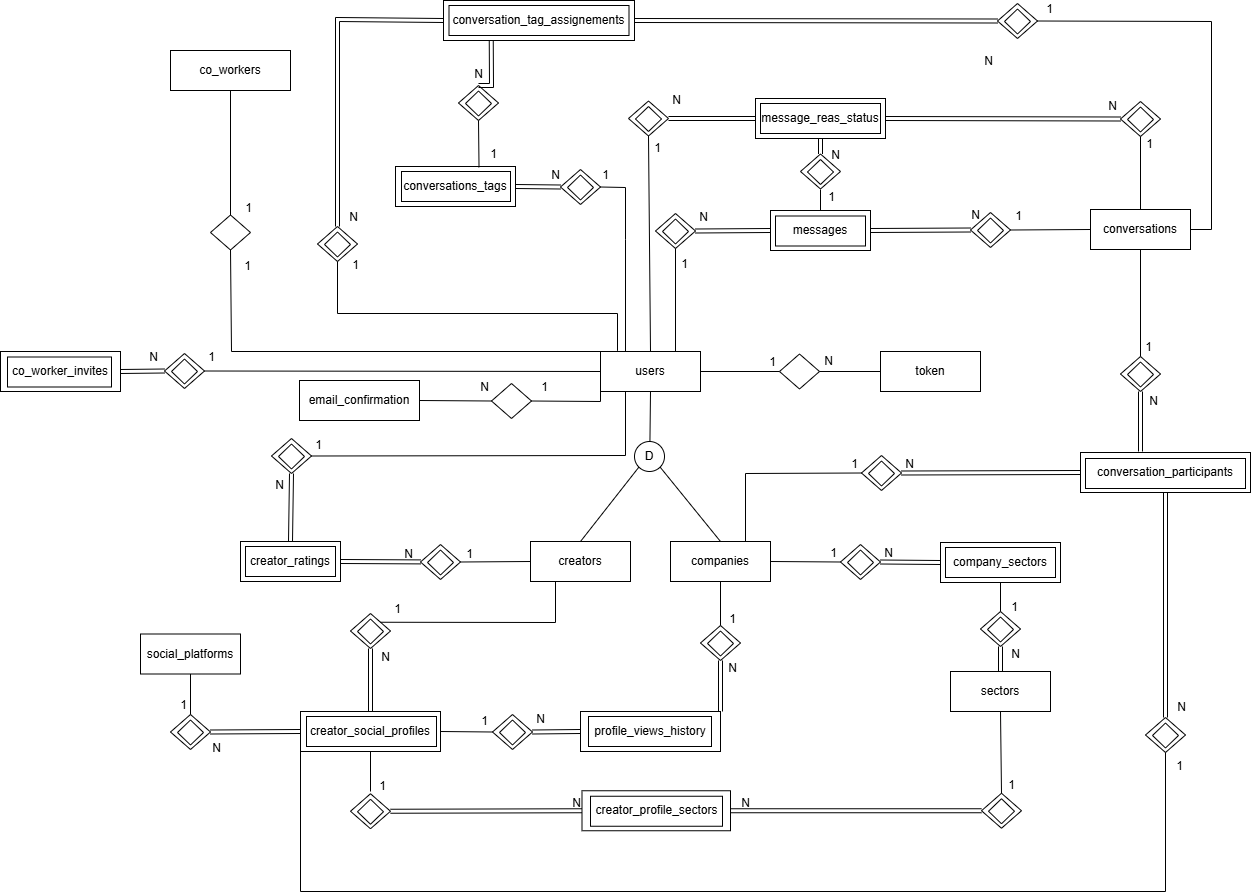
\includegraphics[width=1.3\textwidth]{./img/SimpleERModel.png}
    }
    \caption{Database Structure without attributes, Check complete ER Model on Appendix \ref{fig:er_model}}
    \label{fig:database_structure}
\end{figure}

\begin{figure}[H]
    \centering
    \begin{subfigure}[b]{\textwidth}
        \centering
        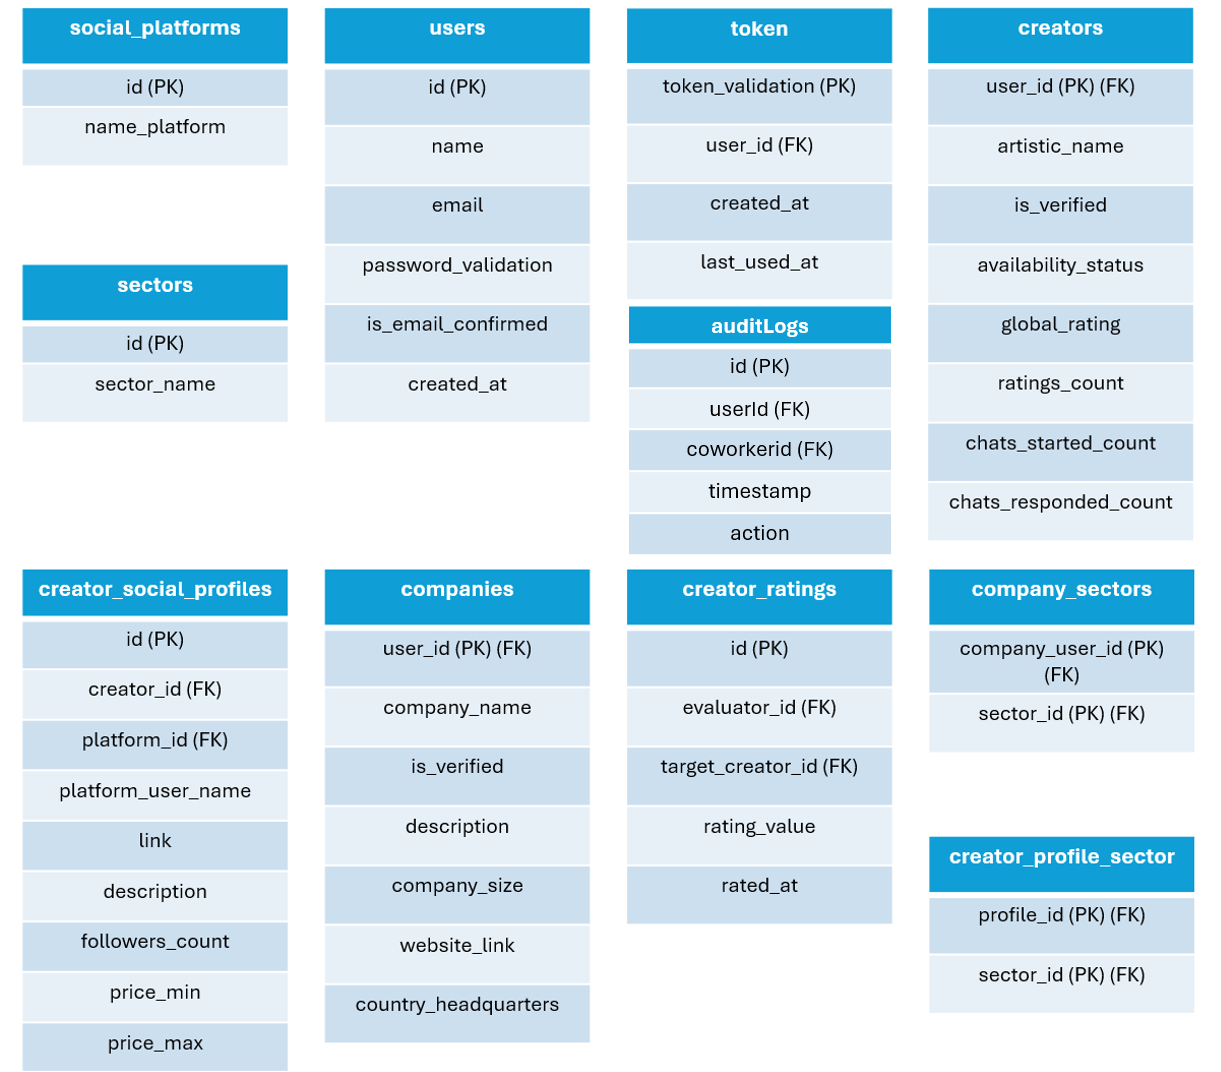
\includegraphics[width=1\textwidth]{./img/table_1.png}
        \caption{Atributte Table 1}
        \label{fig:sub:table1}
    \end{subfigure}


    \begin{subfigure}[b]{\textwidth}
        \centering
        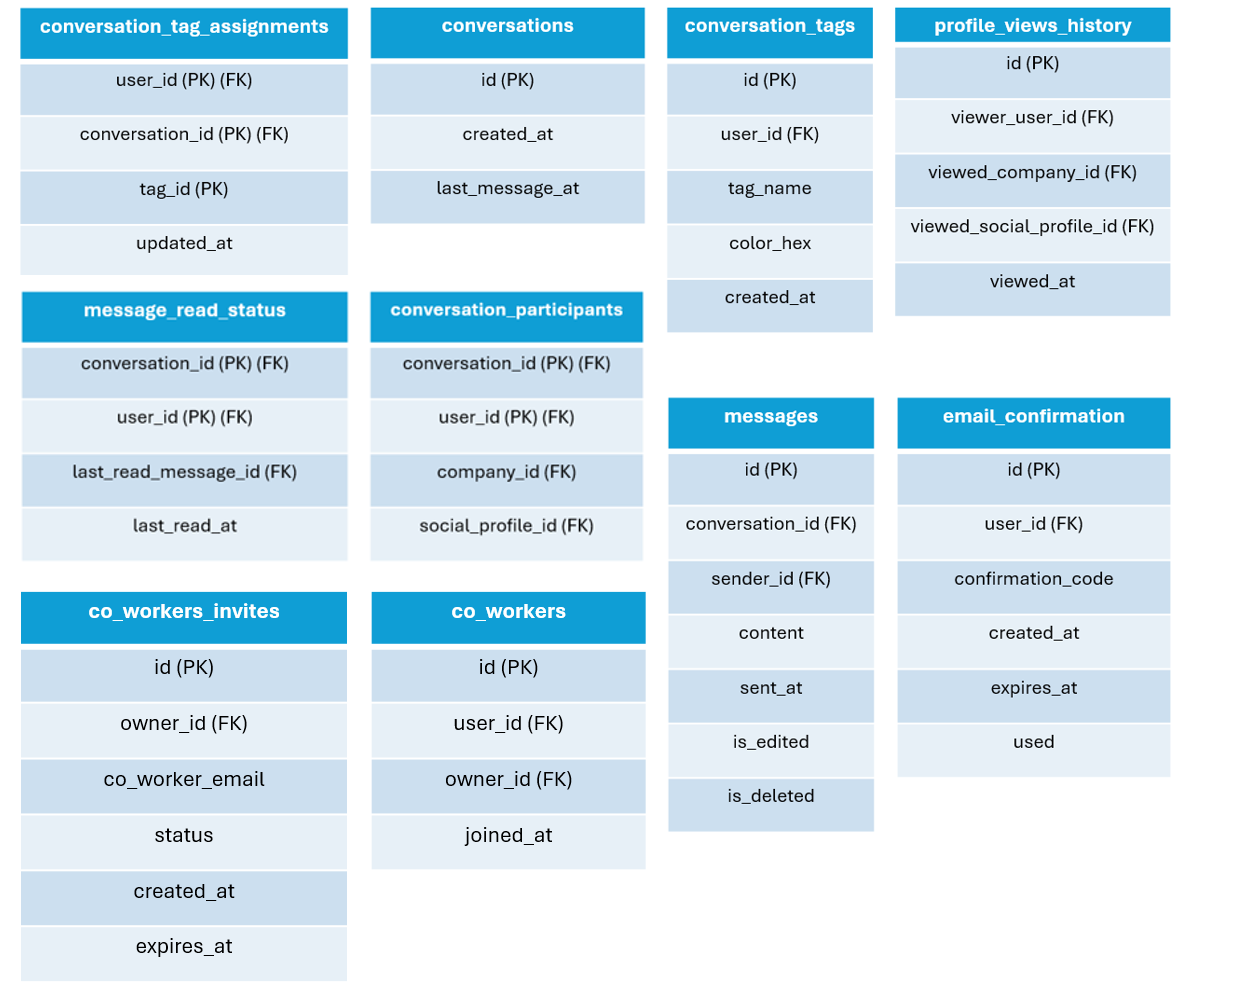
\includegraphics[width=1\textwidth]{./img/table_2.png}
        \caption{Atributte Table 2}
        \label{fig:sub:table2}
    \end{subfigure}
    \caption{Attributes of every entity in the database}
    \label{fig:database_tables}
\end{figure}

The relational model was designed to support the functional and structural needs of a marketplace platform. Each entity and its attributes were carefully selected to reflect real-world concepts such as users, wallets, transactions, goals, and access control. Below is an intuitive justification for the key design decisions:
\begin{itemize}
    \item \textbf{USER}: Represents individual users of the platform. Attributes like email, username, and password\_hash are essential for authentication. The flags is\_email\_confirmed and timestamps help with account lifecycle management.

    \item \textbf{WALLET}: A wallet groups financial data and can be shared among multiple users. It includes balance, currency, and optional description, supporting both individual and group financial tracking.

    \item \textbf{USER\_WALLET}: Models a many-to-many relationship between users and wallets, with an is\_owner flag to distinguish between owners and invited participants.

    \item \textbf{INVITE}: Captures the invitation flow when users are invited to join wallets. The status and joined\_at fields allow tracking of invitation state over time.

    \item \textbf{TOKEN}: Stores session or login tokens for users. Includes created\_at and last\_used\_at to support expiration and activity tracking, promoting secure authentication.

    \item \textbf{EMAIL\_CONFIRMATION}: Used during account creation, storing a unique code, its expiration, and usage status for email verification workflows.

    \item \textbf{ICON} and \textbf{CATEGORY}: Categories help classify transactions (e.g., Groceries, Rent). Each category may be linked to an icon for UI clarity, and the is\_default flag identifies system-defined options. Color and icon references support user personalization.

    \item \textbf{WALLET\_CATEGORY}: Allows each wallet to customize which categories are available, ensuring separation between shared and personal classification systems.

    \item \textbf{TRANSACTION}: Central to the platform, each transaction records amount, type (e.g., income, expense, save), associated wallet, user, category, and optionally links to a saving goal or recurrence rule.

    \item \textbf{SAVING\_GOALS}: Lets users define goals like \emph{Vacation Fund} with a target\_amount, balance, deadline, and status. Tied to a wallet to allow shared or personal goals.

    \item \textbf{RECURRENCE}: Abstracts recurring transaction logic with fields such as recurring\_period, next\_occurrence\_date, and ocurrences\_count. Linked to TRANSACTION when applicable.

    \item \textbf{LIMIT}: Enables setting monthly or weekly spending limits per wallet (and optionally per category). It tracks the current\_amount spent and the limit\_amount, helping users stay on budget.
\end{itemize}

\section{Triggers and Functions}
To help us have less code and unnecessary logic on the API we decided to make some automatic actions on the database using triggers and functions. This helped us to have a more efficient and cleaner code, and also not have to worry about specific logic.

\subsection{Trigger for updating the limit amount when transaction is created}
This trigger is responsible for automatically updating spending limits when a new transaction is recorded in the system. Our application allows users to create spending limits that establish boundaries on the amount of money they can spend, either within specific categories or across all categories (total limit).

When a transaction is created, the trigger performs the following actions:
\begin{itemize}
    \item Checks if there exists any limit associated with the transaction's category and/or a total spending limit.
    \item If a limit exists, verifies whether it has expired. If expired, the trigger marks that limit as inactive and creates a new one. This verification serves as a failsafe, though it should rarely be needed since scheduled tasks regularly check for and handle expired limits.
    \item Updates the current accumulated amount of the relevant limits to reflect the new transaction.
\end{itemize}

For example, if a user has set a monthly limit of \$500 for \emph{Food} category and makes a new purchase of \$50 in that category, the trigger automatically increases the current accumulated amount for that limit from, say, \$200 to \$250, ensuring the user can always see how much of their limit they've used.

\sloppy
Figure~\ref{fig:create_limit_trigger} illustrates this process, showing how the trigger affects the spending limits when a new expense transaction is created. The diagram shows the state of the category limit and total limit before and after the transaction is recorded in the system.

\begin{figure}[H]
    \centering
    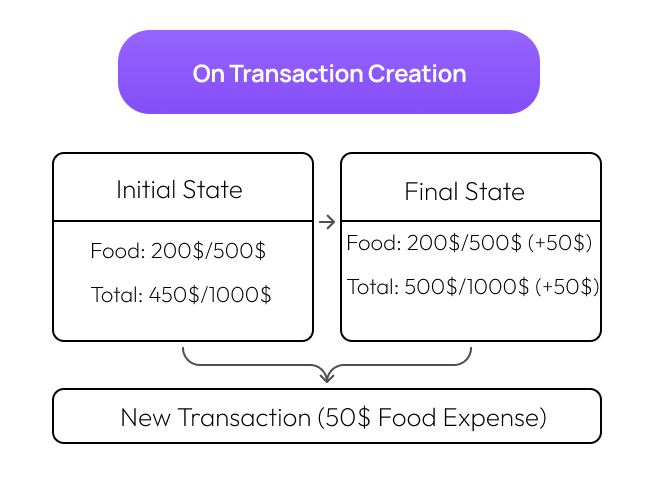
\includegraphics[width=8cm]{img/trigger_on_transaction_create.png}
    \caption{Process of updating limits when a new expense transaction is created.}
    \label{fig:create_limit_trigger}
\end{figure}

\subsection{Trigger for updating the limit amount when transaction is updated}
This trigger manages the recalculation of spending limits when an existing transaction is modified. It uses a straightforward approach to ensure limits remain accurate regardless of what aspects of the transaction were changed.

When a transaction is updated, the trigger executes this process:
\begin{itemize}
    \item First, if the original transaction was an expense, it completely removes the transaction's impact from both the total limit and the category-specific limit.
    \item Then, if the updated transaction is still an expense, it adds the new transaction value to both the total limit and the new category's limit.
\end{itemize}

This two-step approach effectively treats the update as a deletion of the old transaction followed by an insertion of the new one. It handles all possible modification scenarios including:
\begin{itemize}
    \item Changes to the transaction amount
    \item Changes to the transaction category
    \item Changes to the transaction type (from expense to income or vice versa)
    \item Any combination of the above changes
\end{itemize}

For example, if a user changes a \$75 \emph{Entertainment} expense to a \$100 \emph{Dining} expense, the trigger first subtracts \$75 from the \emph{Entertainment} limit and the total limit, then adds \$100 to the \emph{Dining} limit and the total limit.

Figure~\ref{fig:update_limit_trigger} illustrates this update process, showing how the trigger manages changes to limits when a transaction is modified. The diagram demonstrates the complete flow of the operation, from the initial state to the final state, including all intermediate steps of removing and adding values.

\begin{figure}[H]
    \centering
    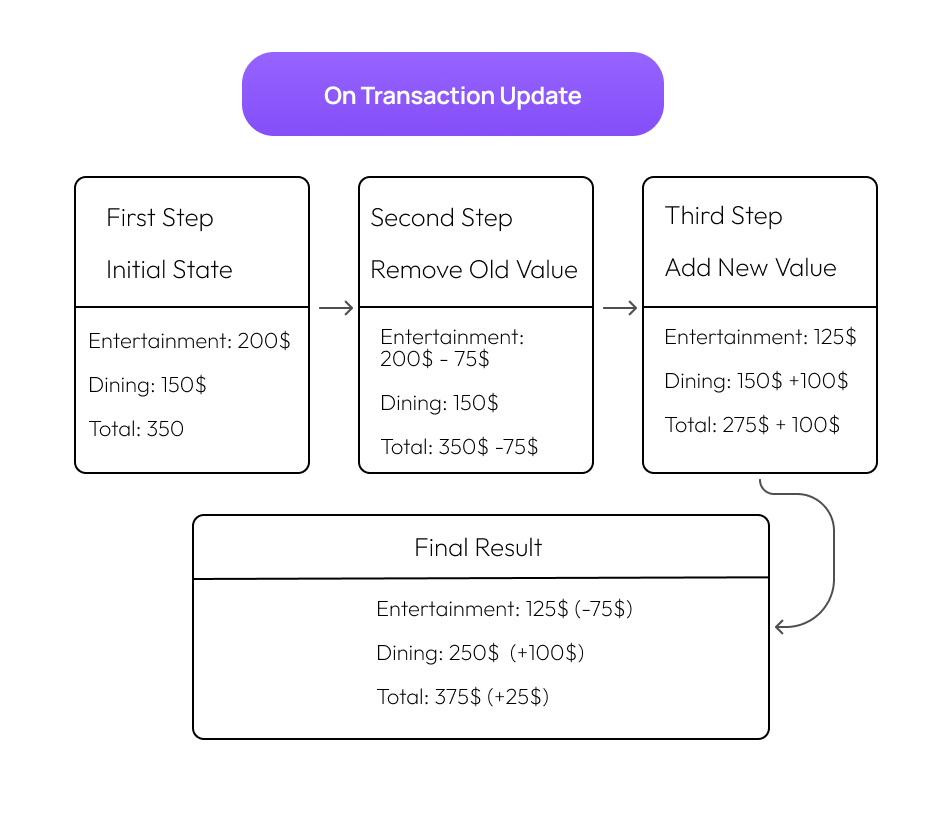
\includegraphics[width=8cm]{img/trigger_on_transaction_update.png}
    \caption{Process of updating limits when a transaction is edited to other category with a diferent amount}
    \label{fig:update_limit_trigger}
\end{figure}


\subsection{Trigger for updating the limit amount when transaction is deleted}
This trigger manages the adjustment of spending limits when a transaction is removed from the system. Deleting transactions requires recalculating the associated spending limits to maintain accurate budget tracking.

When a transaction is deleted, the trigger performs these operations:
\begin{itemize}
    \sloppy
    \item Identifies which spending limits are affected by the deleted transaction (category-specific and/or total limits).
    \item Verifies that these limits are still active and not expired.
    \item Decreases the accumulated amount of each affected limit by the transaction amount, effectively \emph{giving back} the spent amount to the user's available budget.
    \item Ensures that the limit's current amount doesn't fall below zero after the adjustment.
\end{itemize}

For instance, if a user mistakenly recorded a \$120 grocery purchase and later deletes it, the trigger automatically reduces the accumulated amount in their \emph{Groceries} limit by \$120. If their limit was previously at \$350 out of \$500, it would now show \$230, correctly reflecting that they have more available budget than previously indicated.

Figure~\ref{fig:delete_limit_trigger} illustrates this process, showing how the trigger adjusts the spending limits when a transaction is deleted. The diagram demonstrates how the removal of a transaction leads to the corresponding reduction in the accumulated amounts for both the category-specific limit and the total spending limit.

\begin{figure}[H]
    \centering
    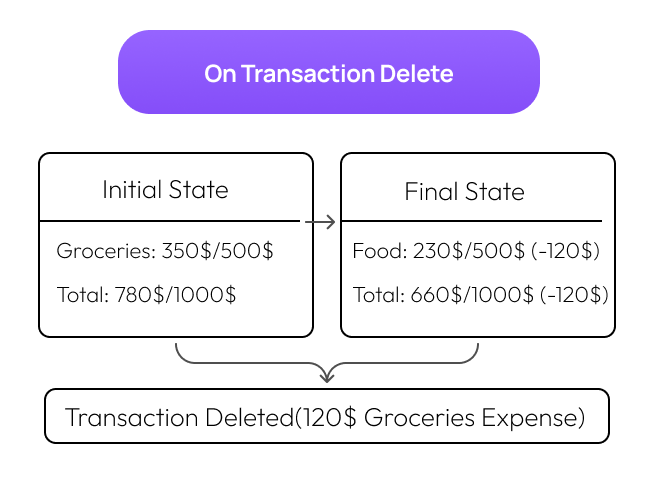
\includegraphics[width=9cm]{img/trigger_on_transaction_delete.png}
    \caption{Process of updating limits when a transaction is deleted}
    \label{fig:delete_limit_trigger}
\end{figure}

\subsection{Trigger for adding default categories to a new wallet}
This trigger simplifies the wallet setup process by automatically associating newly created wallets with a predefined set of categories. This ensures users can immediately begin tracking their expenses without having to manually configure categories.

For example, when a user creates a new wallet, it will automatically be configured with the default categories like \emph{Food}, \emph{Transportation}, \emph{Housing}, \emph{Entertainment}, and \emph{Utilities}. This means the user can immediately begin categorizing their transactions without any additional setup.

This automatic initialization improves the user experience by reducing the initial configuration required and ensuring consistency across wallet setups. Users can still customize their categories later by adding new ones that make more sense for their specific needs.

\chapter{Web Frontend Architecture}\label{ch:frontend_web}

This chapter explores the frontend ecosystem of the project, outlining its architectural design and highlighting the implementation of its core features.

\section{Frontend Structure}

\begin{figure}[H]
    \centering
    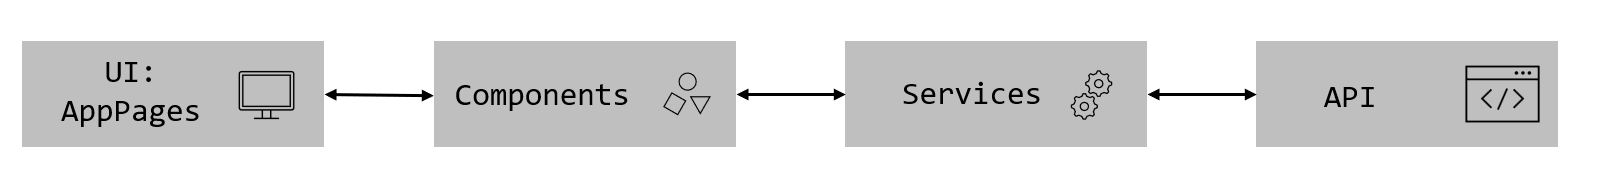
\includegraphics[width=1.05\textwidth]{img/frontend_structure.png}
    \caption{Frontend Structure}
    \label{fig:web-frontend-structure}
\end{figure}

The frontend structure is organized into three main directories:
\begin{itemize}
    \item \textbf{app:} This directory contains the main application logic, routing, and top-level components that orchestrate the application flow.
    \item \textbf{components:} This directory is dedicated to reusable UI elements and some specific components that are used in the application.
    \item \textbf{services:} This directory handles business logic, data fetching, interactions with the backend API, and other functionalities that need to be shared or separated from the UI components.
\end{itemize}


\section{Components}
The components are the main building blocks of the frontend. They are used to create the UI of the application, they are not associated with a specific page which means they are reusable.

They are organized in the \texttt{components} directory, when one is used in multiple pages it is placed in the \texttt{ui} directory, these ui components are mainly imported from shadcn/ui. The components are organized by the page they are used in, for example the \texttt{dashboard} directory contains components used in the dashboard page like the \texttt{walletOverview} and \texttt{expenseChartItem} components.


\subsection{State Management}
Our application relies on a structured state management approach to ensure data consistency and component reactivity. We implemented a hybrid strategy combining local component state with global application state management.

At the component level, we leverage React's useState hook for managing local state such as form inputs, loading states, and temporary UI interactions. For application-wide state that needs to be shared across multiple components, we implemented a context-based architecture using React's useContext hook.

The core of our global state management centers around the \texttt{WalletContext}, a custom context provider that maintains the user's wallet collection and tracks the currently selected wallet. This centralized approach ensures that wallet-related data remains synchronized across all components that depend on it. See more details on the context implementation in Section \ref{sec:contexts_web}.

We deliberately chose this combination over more complex state management solutions like Redux or state machines. While state machines offer powerful state transition control, our use case primarily involves managing straightforward data flows and form states. The useState approach provides sufficient flexibility for handling complex forms, such as the transaction creation form, where we manage both service-fetched data and user input validation simultaneously.

\subsection{Components Interaction}
The components are organized in a way that allows them to interact with each other. For example, the \texttt{limits} component uses the \texttt{limitsCarousel} component to display the limits of the different categories. In this case the \texttt{limits} component is the parent and the \texttt{limitsCarousel} component is the child, which means that all the data that the \texttt{limitsCarousel} component needs is passed as props in the \texttt{limits} component, sometimes callbacks are passed to the child component to handle the user interactions as shown in the example below.

\begin{lstlisting}[caption={Limits Component child component}, label={lst:limits-component-child}]
<LimitCarousel
    limits={limits}
    onEditClick={handleEditClick}
    onDeleteClick={handleDeleteClick}
/>
\end{lstlisting}

This way the father component has the ability to control the child appearance and behavior through props. When there are new information to be displayed in the child component, the father component can pass the new information as props and the child component will be able to use it to render the new information.

\subsection{API Interactions}
In order for the components to have the data they should display, they need to call the services that fetch the data from the API. This is done by using the useEffect hook, which is a hook that is used to fetch the data when the component is mounted or when a specific state of the component changes. The next example shows how the \texttt{limits} component fetches the data from the API.

\begin{lstlisting}[caption={Limits Component useEffect}, label={lst:limits-component-useEffect}]
useEffect(() => {
    setIsLoading(true);
    const fetchData = async () => {
        try {
            const [newLimits, categories] = await Promise.all([
                limitService.getLimits(walletId, limit, offset),
                CategoryService.getCategories(walletId)
            ]);
            setLimits(newLimits);
            setAllCategories(categories);
        } catch (error) {
            console.error("Error fetching data:", error);
        } finally {
            setIsLoading(false);
        }
    };
    fetchData();
}, []);
\end{lstlisting}

\section{Report}

To provide users with better control over their finances, we implemented a customizable report generation feature using PDF generation. Before addressing the technical implementation, we first decided between client-side and server-side approaches. We chose client-side generation for several reasons: it reduces server load, enables real-time user feedback during the generation process (displaying progress indicators like "fetching transactions", "processing categories", "generating charts"), and offers better scalability for an application with potentially many users generating reports concurrently.

With this decision made, we then faced the challenge of incorporating graphics into PDFs. After research and testing, we considered the two most common approaches:
\newpage
\begin{itemize}
    \item \textbf{Approach 1: Render graphics in the DOM and capture them as images for the PDF.} \\
    This method involves creating the visualizations using standard rendering techniques (e.g., charts via libraries like Recharts or Chart.js), taking a screenshot of them (e.g., with \texttt{html2canvas}), and embedding the resulting image in the PDF. We also found some personal projects from developers who faced the same problem and created libraries to automate this process. However, since these libraries could be discontinued or their usage might be restricted in the future, we decided not to consider them.

    \textbf{Pros:}
    \begin{itemize}
        \item Faster to implement, as it leverages existing visualization libraries.
        \item Minimal need to manually manage graphical layout or rendering logic.
    \end{itemize}
    
    \textbf{Cons:}
    \begin{itemize}
        \item Unreliable results: screenshots often failed or captured incomplete content.
        \item Lower quality and resolution, especially when scaling or printing.
        \item Limited styling control once the image is captured.
    \end{itemize}
    
    \item \textbf{Approach 2: Generate graphics directly in SVG and include them in the PDF.} \\
    This alternative involves writing logic to build and render the graphics directly as SVG elements, which are then embedded into the PDF.

    \textbf{Pros:}
    \begin{itemize}
        \item Full control over layout, styling, and rendering.
        \item High-quality output that scales well for printing.
        \item More reliable and consistent integration into the PDF.
    \end{itemize}
    
    \textbf{Cons:}
    \begin{itemize}
        \item Requires additional development effort to implement custom rendering logic.
        \item Increased complexity when we need advanced visuals(pie charts, bar charts, etc).
    \end{itemize}
\end{itemize}

After evaluating both approaches, we opted for the second one due to its superior flexibility, quality, and reliability—despite the extra development effort required to manually build the SVG graphics.




\section{Contexts} \label{sec:contexts_web}
In the React framework, contexts are used to share data between components without the need to pass props through the entire component tree. This is especially useful when the same data needs to be accessed across multiple views. In our implementation, we use several contexts, but the most important one is the \texttt{WalletContext}, which stores both the selected wallet and the list of all wallets belonging to the user. This is essential because most of our main components need access to this data.

We treat this context like a cache, allowing us to access wallet information without making repeated API calls. This is particularly helpful on the dashboard page, where wallet data needs to be available at all times.

To implement this properly, we created a \texttt{WalletProvider} component. It wraps the parts of the application that need access to the wallet context. This component handles the state for both the wallets and the selected wallet. It fetches data from the API, stores it in the context, and provides it to the components that depend on it. Here's what the return statement of the \texttt{WalletProvider} component looks like:

\begin{lstlisting}[caption={WalletProvider}, label={lst:wallet-provider}]
    return (
        <WalletContext.Provider
          value={{
            currentWallet: currentWallet!,
            wallets,
            loading,
            changeWallet,
            changeBalance,
            editWallet,
            deleteWallet,
            ...
          }}
        >
          {children}
        </WalletContext.Provider>
      );
\end{lstlisting}

As shown above, the \texttt{WalletProvider} component returns a \texttt{WalletContext.Provider}, which supplies the selected wallet, all wallets, and a set of functions to manage them. When the provider is mounted, it fetches the wallets from the API and stores them in the context.

To make it easier to use this context in components, we also created a custom hook called \texttt{useWallet}. This hook allows components to access wallet data without having to directly use \texttt{useContext(WalletContext)}. Here's an example of how it's used:

\begin{lstlisting}[caption={useWallet}, label={lst:use-wallet}]
const { currentWallet, wallets, loading, changeWallet, changeBalance, editWallet, deleteWallet } = useWallet();
\end{lstlisting}

The useWallet hook was created so the components that need to access the wallets or the selected wallet can do it without having to use the \texttt{useContext(WalletContext)}. Here is the implementation of the useWallet hook.

\begin{lstlisting}[caption={useWallet hook}, label={lst:use-wallet-hook}]
    export const useWallet = (): WalletContextType => {
        const ctx = useContext(WalletContext);
        if (!ctx) {
          throw new Error('useWallet must be used within WalletProvider');
        }
        return ctx;
      };
\end{lstlisting}

There are other contexts that are used in the application such as: 

\begin{itemize}
    \item \texttt{RegisterContext} that is used to store the email of the user when the user is registering.
    \item \texttt{ThemeContext} that is used to store the theme of the application.
\end{itemize}

\section{Middleware}
To help user experience and prevent unauthorized access to protected frontend pages, we implement a Next.js middleware\cite{nextjs-middleware} that handles authentication-based routing decisions. This middleware operates exclusively on frontend page routes, ensuring users are properly directed based on their authentication status without interfering with API endpoint functionality, this middleware only checks if the token exists in the cookies and if it does it redirects to the dashboard page and then the backend checks if the token is valid, since we can't have the value of the cookies via typescript, if the token does not exist it redirects to the home page.

\begin{lstlisting}[caption={Middleware}, label={lst:middleware_frontend_web}]
const publicRoutes = ['/', '/register', '/register/confirmEmail'];

export function middleware(request: NextRequest) {
    const { pathname } = request.nextUrl;
    const isPublicRoute = publicRoutes.some(route => pathname === route);
    const token = request.cookies.get('token')?.value;

    if (!isPublicRoute && !token) {
    return NextResponse.redirect(new URL('/', request.url));
    }

    if ((pathname === '/' || pathname === '/register') && token) {
    return NextResponse.redirect(new URL('/dashboard', request.url));
    }

    return NextResponse.next();
}

export const config = {
    matcher: ['/((?!api|_next|.*\\..*).*)'],
};
\end{lstlisting}

The middleware intercepts requests to frontend pages and evaluates the user's authentication status through cookie-stored tokens. It automatically redirects users to appropriate pages based on their authentication state, creating a seamless navigation experience while maintaining security boundaries for protected content.

\textbf{Important Note:} This middleware specifically excludes API routes (as defined by the matcher configuration). The middleware focuses solely on frontend page routing and user experience optimization.

\subsection{Architecture Components}
\textbf{Route Classification System:}
The publicRoutes array defines frontend pages accessible without authentication, including the home page (/), user registration (/register), and email confirmation (/register/confirmEmail) routes. This centralized configuration allows for easy modification of public access permissions as the application grows.

\textbf{Selective Route Matching:}
The matcher configuration ensures the middleware only processes frontend page requests while excluding:
\begin{itemize}
\item API routes (\texttt{/api/*})
\item Next.js internal routes (\texttt{/\_next/*})
\item Static assets (files with extensions like \texttt{.css}, \texttt{.js}, \texttt{.png}, etc.)
\end{itemize}
This selective approach prevents interference with API functionality and static resource serving.

\textbf{Token-Based Authentication Check:}
The middleware extracts authentication tokens from HTTP cookies to determine user authentication status. This approach provides a server-side validation mechanism that works seamlessly with Next.js's server-side rendering capabilities.

\textbf{Intelligent Page Redirection:}
The system implements smart redirection logic for optimal user experience:
\begin{itemize}
\item Unauthenticated Access Protection: Users without valid tokens attempting to access protected frontend pages are redirected to the home/login page, preventing access to sensitive areas like user dashboards or account pages.
\item Authentication Flow Optimization: Users with valid tokens who navigate to login or registration pages are automatically redirected to the dashboard, eliminating redundant authentication steps and improving user flow.
\end{itemize}

\textbf{Request Continuation:}
When no redirection conditions are met, the middleware allows requests to proceed normally using NextResponse.next(), maintaining standard Next.js routing behavior for all appropriate scenarios.

This middleware architecture focuses specifically on frontend user experience and page-level access control, while API security remains the responsibility of individual endpoint implementations.
\chapter{Tests}\label{ch:tests}

\paragraph{}This chapter details the testing strategies and procedures performed on the project, covering just backend components.

\section{Backend Tests} \label{sec:backend_tests}
We adopted a layered testing approach to ensure high confidence in our system’s behavior. With some tests written across the solution, our goal was to validate that every function in the application performs exactly as intended — both in isolation and when integrated with other core sub-systems. This rigorous test coverage helps us identify regressions early, improve maintainability, and confidently refactor our codebase during agile iterations.

\subsubsection{Unit Tests}
For the domain logic residing in our Service Layer, we wrote extensive unit tests using Moq to isolate external system behaviors, such as database repositories and cross-cutting infrastructure concerns. These tests validate:

\begin{itemize}
    \item Strict domain validation rules (e.g., preventing empty, white-spaced, or overly long conversation tag names).
    \item Behavior under diverse edge cases (e.g., attempting to tag a conversation where the user is not an active participant, or manipulating tags that belong to other identities).
    \item Error routing integrity using explicit strongly-typed results via the \texttt{OneOf} library pattern.
\end{itemize}

To keep our test suites maintainable, clean, and fast, we structured them using XUnit's \texttt{IClassFixture<T>} interface. We established a reusable fixture class for each core service lifecycle, such as the \texttt{ConversationTagServiceFixture}.

\begin{lstlisting}[caption={ConversationTagServiceFixture instantiation}, label={lst:conversation-tag-fixture-init}]
public class ConversationTagServiceTests : IClassFixture<ConversationTagServiceFixture>
\end{lstlisting}

Implementing centralized class fixtures yields significant advantages:
\begin{itemize}
    \item \textbf{Decoupled Mock Orchestration:} Pre-configures interconnected dependency graphs, mock states, and multi-repository contexts (such as \texttt{IConversationTagRepository}, \texttt{IUserRepository}, and \texttt{IConversationRepository}) within a centralized setup constructor.
    \item \textbf{Transactional Context Management:} Simulates nested transactional boundaries through specialized manager wrappers (\texttt{ITransactionManager}), mirroring real production database behaviors.
    \item \textbf{State Fluidity Utilities:} Exposes intuitive helper states (e.g., \texttt{SetupTagNameExists(bool)}, \texttt{SetupUserIsParticipant(bool)}) that let individual test cases manipulate mock flows cleanly using declarative state shifts.
\end{itemize}

\begin{lstlisting}[caption={Unit test execution inside ConversationTagServiceTests}, label={lst:conversation-tag-unit-tests}]
[Fact]
public async Task CreateTag_ShouldReturnError_WhenTagNameAlreadyExists()
{
    // Arrange
    _fixture.SetupUserExists(true);
    _fixture.SetupTagNameExists(true);
    _fixture.SetupCreateTag(10);

    // Act
    var result = await _fixture.ConversationTagService.CreateTag(_fixture.UserId, "Duplicada", "#FFFFFF");

    // Assert
    Assert.True(result.IsT1); // Validates that a failure union state was reached
    Assert.IsType<ConversationTagError.TagNameAlreadyExists>(result.AsT1);
}
\end{lstlisting}

As illustrated in Listing~\ref{lst:conversation-tag-unit-tests}, our test execution relies on declarative setup triggers. By feeding a pre-existing tag scenario into the mock layers, the service execution triggers a failure branches inside the domain validation. Instead of throwing raw exceptions, the application uses discriminated unions (\texttt{OneOf}) to output functional result branches. 

The test structure easily intercepts this by asserting that the response is mapped to the failure index state (\texttt{IsT1}) and confirms the dynamic payload matches the specific architectural error class (\texttt{ConversationTagError.TagNameAlreadyExists}).

\chapter{AI Integration}\label{ch:ai}
\paragraph{}This chapter focuses on the integration of artificial intelligence techniques into the Hubly system and how we used the AI.


\paragraph{}Artificial intelligence tools were used during the development of this project as support tools, mainly for writing, clarification and code assistance. Their use was auxiliary and did not replace the team's decision-making process, technical implementation or validation of the final solution.

\paragraph{}In the written report, AI tools were used to support the improvement of English writing, sentence structure and academic tone. They were also used to help complete or reorganize ideas when describing technical concepts, ensuring that the explanations were clearer and more consistent with the structure of the report.

\paragraph{}During the implementation phase, AI tools were also used as support for code-related tasks. This included help with code organization, identification of possible improvements, code optimization suggestions and the creation or improvement of comments. All generated suggestions were reviewed, adapted and validated by the team before being included in the final project.

\paragraph{}\textbf{Model of the AI and version}

\begin{itemize}

\item \textbf{ChatGPT:} ChatGPT Plus - GPT-4.5 Thinking

\item \textbf{Gemini:} Gemini 3.1 Flash-Lite

\end{itemize}

\chapter{Conclusion}\label{ch:conclusion}

\paragraph{}As this project reaches its completion, Hubly can be considered to have fulfilled the main objectives defined at the beginning of the work. The project involved the development of a full-stack web application using .NET for the backend, PostgreSQL for the relational database, and React/Next.js for the web frontend. This technology stack presented several technical challenges, but it also provided an opportunity to understand the interaction between backend services, database design and frontend application development in a web application context.

Developing Hubly allowed us to apply and expand the theoretical knowledge acquired throughout the academic program, connecting computer engineering concepts with the design of a marketplace-oriented application. The project also provided experience with different development paradigms, such as the typed backend architecture of .NET and the component-based structure of React. Working with these technologies contributed to the development of full-stack skills, problem-solving abilities and a better understanding of how different system components interact within a complete application.

The implementation of Hubly required addressing several software engineering and architectural challenges. One relevant aspect was the design of the relational database schema, where a single user can act as a company or as a creator with multiple social profiles. Each social profile required its own metadata, messaging context and private conversation tags. Another important component was the implementation of multi-criteria search mechanisms for both \emph{CreatorSearchInputModel} and \emph{CompanySearchInputModel}, allowing users to filter results according to sectors, price ranges, audience size, company size and location. In addition, the internal messaging system was designed to associate conversations with specific company or creator social profiles, rather than only with generic user accounts. The system also includes profile-view history and recommendation logic, which provide a basis for suggesting companies or creator social profiles according to previous interactions.

Looking forward, Hubly could be extended in several ways. Future work may include the integration of social media APIs, such as Meta and YouTube APIs, to support audience verification, metric collection and demographic data retrieval. Another possible improvement would be the implementation of a multi-user collaboration system, allowing marketing or management teams to administer the same company or creator profile. To support this type of shared access, concurrency control mechanisms, such as optimistic locking, could be introduced to prevent conflicts when multiple users modify the same information. An audit logging system could also be added to record relevant user actions, including the user responsible for the action, the affected area of the application and the corresponding timestamp.

Overall, Hubly provides a structured solution for supporting interactions between companies and digital creators. By centralizing profile discovery, profile-based conversations and private negotiation tags, the system reduces dependence on scattered external communication channels. The final prototype demonstrates how a web application can support company-creator partnerships through organized search, communication and interaction tracking workflows.


\bibliographystyle{unsrt}
\bibliography{references}
\addcontentsline{toc}{chapter}{References}

\appendix
\chapter{Complete ER Model}
\label{app:er_model}

\begin{figure}[H]
    \centering
    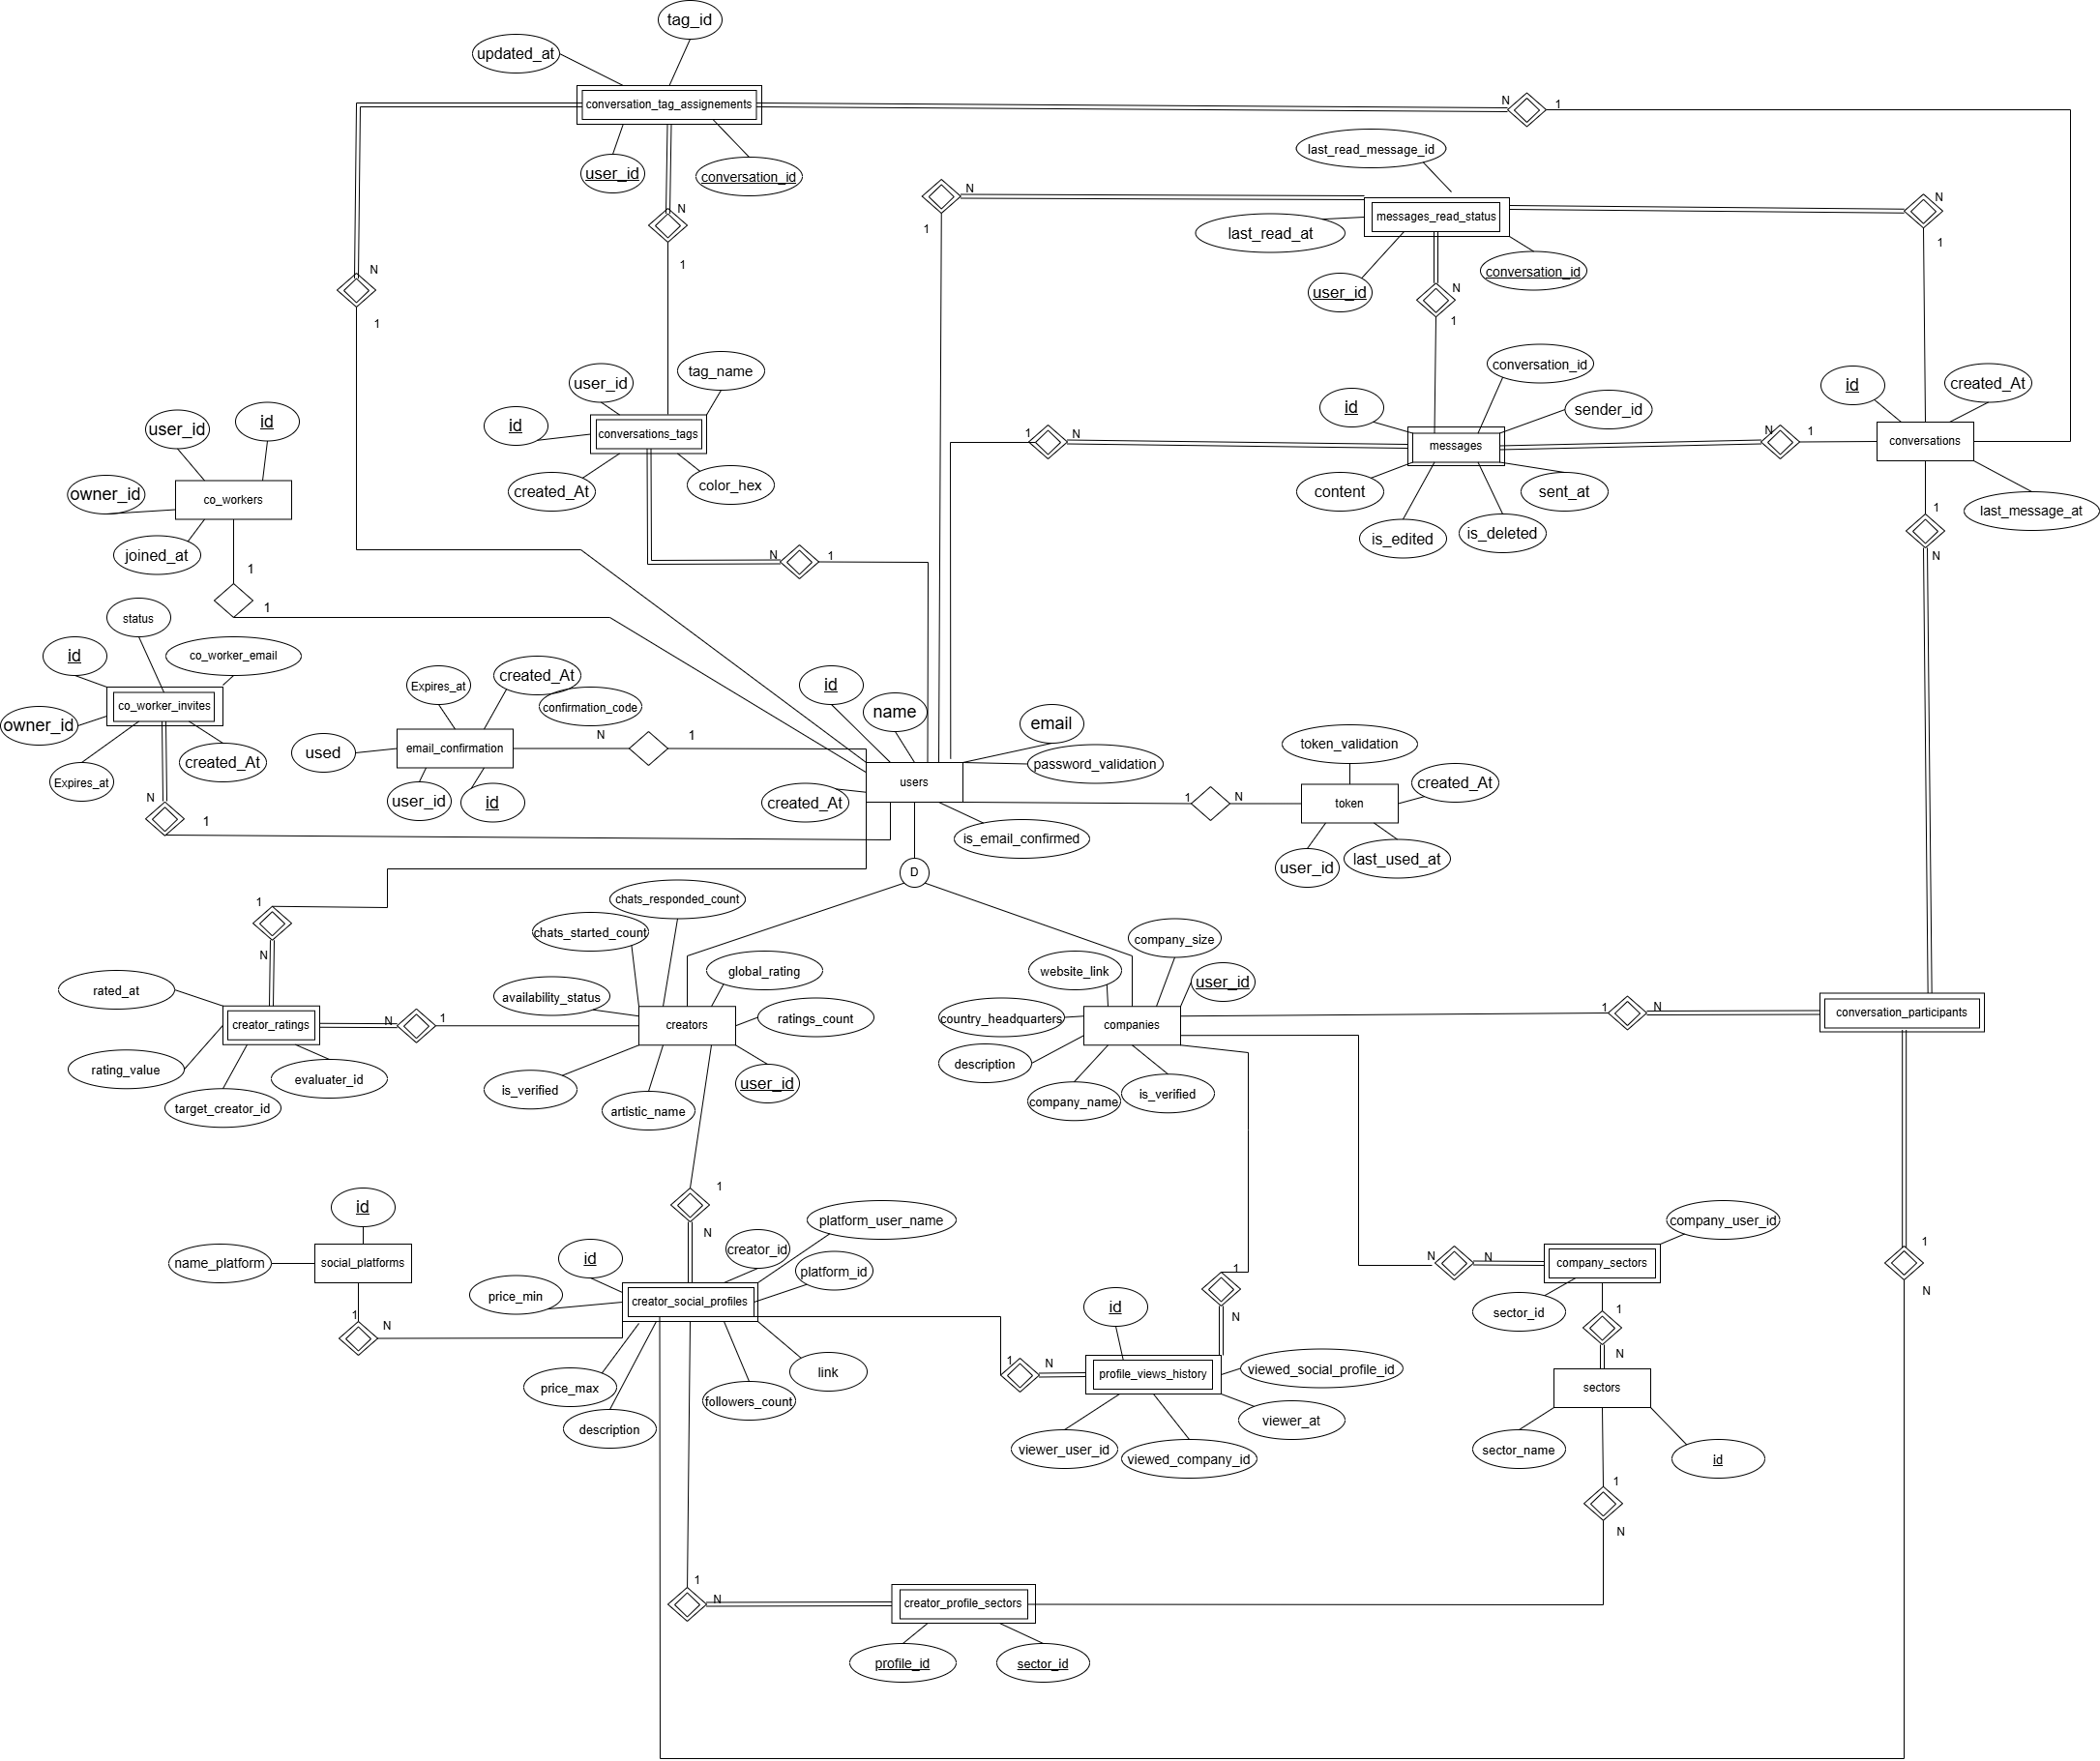
\includegraphics[width=1.1\textwidth]{./img/ERModel.png}
    \caption{Complete ER Model}
    \label{fig:er_model}
\end{figure}

\end{document}